\chapter{随机变量列的收敛}
\label{chap:random-variable-convergence}

反复从$[0,1)$中均匀地随机取数，记下前$n$个数中的最大值$M_n$。取的数越多，最大值越接近$1$，这一点很少有人怀疑。可是“$M_n$趋于$1$”到底说的是什么？$M_n$不是一个数，而是随抽取结果变化的随机变量；说它“趋于”某个值，必须先说清楚在什么意义下比较它与目标的差。

至少有三种自然的读法。第一种盯住一次完整的抽取记录：记录固定以后，$M_1,M_2,\dots$是一列普通的数，问这列数是否收敛。第二种固定样本量$n$，问误差超过某个阈值的机会有多大，再看这个机会是否随$n$消失。第三种也固定$n$，但问误差的平均大小，例如平均绝对误差或均方误差是否趋于零。

对$M_n$来说三种读法给出相同的回答，但它们一般并不等价。有的随机变量列误差超标的机会越来越小，却在每一条抽取记录上都反复超标；有的随机变量列在每条记录上最终都归于零，平均误差却始终不变。前者缺的是对整条记录的控制，后者缺的是对稀有大取值的控制。

本章先在同一个概率空间上给出三种收敛方式：几乎必然收敛、依概率收敛和$L^{p}$收敛，并用几个可以手算的例子逐一检验它们之间的蕴含关系与反例。随后研究怎样判断几乎必然收敛：把“误差最终变小”改写为“超差事件只发生有限次”，由此得到Borel–Cantelli引理和子列刻画。最后研究期望能否与极限交换，依次讨论单调性、共同上界和一致可积性各自提供的保证，得到$L^{1}$收敛的判据。

\section{收敛方式}
\label{sec:rvconv-modes}

全章固定一个概率空间$(\Omega,\mathcal{F},\mathbb{P})$，在它上面讨论实随机变量$X_1,X_2,\dots$和一个候选极限$X$，它们都取有限实数值。要问的是$X_n$是否“趋于”$X$，所以把差
\[
 X_n-X
\]
当作共同的研究对象，称为第$n$项的误差。误差本身是$\Omega$上的函数，每个样本点$\omega$给出一个数$X_n(\omega)-X(\omega)$。

“误差趋于零”可以从三个角度提要求。逐样本：固定$\omega$，看数列$X_n(\omega)-X(\omega)$是否趋于零。逐事件：固定$n$和阈值$\varepsilon$，看误差超过$\varepsilon$这一事件的概率。逐平均：固定$n$，看误差绝对值的某次幂的期望。三个角度依次给出本节的三种收敛方式。

函数列的逐点、依测度与$L^{p}$收敛已经在一般测度空间上建立，可参考\BookChapterRef{chap:function-normed-spaces}{卷四第11章“赋范空间”}。本节不重复一般的定义和证明，而是在总质量为一的概率空间上解释每一种要求控制了什么、放过了什么。

\paragraph{贯穿全章的例子}
设$U_1,U_2,\dots$是相互独立的$\operatorname{Unif}(0,1)$随机变量，它们可以定义在同一个概率空间上（独立序列的构造见第~\ref{chap:probability-spaces}章），并记$U=U_1$。由它们构造下面几族随机变量，全章反复使用。第一族是累计最大值，第二族是独立示性变量，其中$p_n\in[0,1]$，$A_n=\{U_n<p_n\}$：
\[
 M_n=\max\{U_1,\dots,U_n\},\qquad \xi_n=\mathbf{1}_{A_n} .
\]
第三族是稀有大值：
\[
 Y_n=n\,\mathbf{1}_{\{U<1/n\}},\qquad Z_n=\sqrt{n}\,\mathbf{1}_{\{U<1/n\}} .
\]
第四族是移动区块$B_n$：第$k$层把$[0,1)$等分为$k$段，依次取各段的示性函数，具体写法见第~\ref{sec:rvconv-convergence-in-probability}小节。$M_n$的候选极限是常数$1$，其余几族的候选极限都是$0$。
$M_n$在三种意义下都收敛，其余几族各在某些意义下不收敛，用来检验各种收敛方式的边界。

\subsection{几乎必然收敛}
\label{sec:rvconv-almost-sure}

先把样本点$\omega$看成一次完整的观测记录。对累计最大值，$\omega$对应一串取值$U_1(\omega),U_2(\omega),\dots$，也就是无限次重复抽取的全部结果；记录一旦确定，$M_1(\omega),M_2(\omega),\dots$就是一列普通的数。图~\ref{fig:rvconv-max-paths}(a)画了五条这样的记录，每条记录上的误差$1-M_n(\omega)$都单调下降，并且迟早落到阈值$\varepsilon=0.1$以下。

\begin{BookInlineFigure}
 \centering
 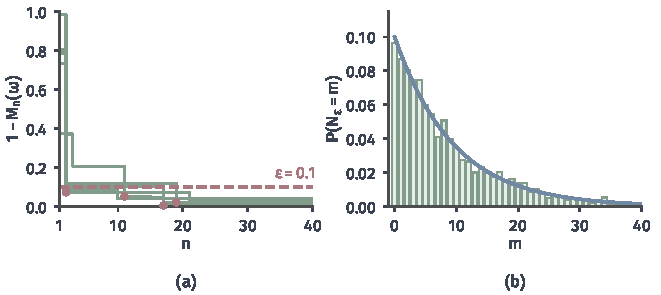
\includegraphics[width=112mm]{figures/07-probability/03-probability-limits/matplotlib/rvconv-max-paths/figure.pdf}
 \caption{累计最大值$M_n=\max\{U_1,\dots,U_n\}$的误差。(a)五条模拟记录上的$1-M_n(\omega)$（绿色台阶，种子$7$），红色虚线为阈值$\varepsilon=0.1$，红点标出误差最后一次降到阈值以下的位置。(b)最后一次超过阈值的序号$N_{\varepsilon}$：浅绿柱为$4000$条模拟记录的频率（种子$11$），蓝线为精确的质量$0.9^{m}\times0.1$。}
 \label{fig:rvconv-max-paths}
\end{BookInlineFigure}

\paragraph{例外的记录}
是不是每一条记录都如此？不是。若一条记录上所有$U_i(\omega)$都不超过$0.9$，比如每次都取到$0.5$，那么$M_n(\omega)\leq0.9$对一切$n$成立，误差永远不小于$0.1$。这样的记录是存在的，问题是它们一共有多大的概率。

$M_n(\omega)$随$n$递增且不超过$1$，所以它总收敛到$\sup_iU_i(\omega)$。它不收敛到$1$，当且仅当$\sup_iU_i(\omega)<1$，也就是存在正整数$k$，使所有$U_i(\omega)\leq1-1/k$。对固定的$k$和任意$n$，由独立性，
\[
 \mathbb{P}\bigl(U_i\leq1-\tfrac1k\text{ 对一切 }i\bigr)\leq\mathbb{P}\bigl(U_1\leq1-\tfrac1k,\dots,U_n\leq1-\tfrac1k\bigr)=\Bigl(1-\frac1k\Bigr)^{n}.
\]
右边随$n\to\infty$趋于零，左边与$n$无关，所以左边为零。再对$k=1,2,\dots$取并，可数个零概率事件的并仍是零概率事件，于是
\[
 \mathbb{P}\bigl(M_n\not\to1\bigr)=0 .
\]
例外的记录确实存在，但它们合在一起的概率为零。

\paragraph{定义}
这正是几乎必然收敛的含义：允许一个零概率的例外集合，在它之外，每条记录上的数列都收敛到目标。

\begin{definition}[几乎必然收敛]
\label{def:rvconv-almost-sure}
若
\begin{equation}
 \mathbb{P}\bigl(\{\omega:X_n(\omega)\to X(\omega)\}\bigr)=1 ,
 \label{eq:rvconv-almost-sure}
\end{equation}
称$X_n$\term{几乎必然收敛}（almost sure convergence）到$X$，记作$X_n\xrightarrow{\mathrm{a.s.}}X$。
\end{definition}

式~\eqref{eq:rvconv-almost-sure}里的集合是由可数次集合运算得到的事件，第~\ref{sec:rvconv-infinitely-often}小节会把它写出来。几乎必然收敛就是卷四所说的几乎处处收敛，只是测度换成了概率：例外集合$\{X_n\not\to X\}$是零概率事件。

\paragraph{同一个例外集}
定义里只有一个例外集合，它要容纳整列不收敛的所有记录。展开来说，存在零概率事件$N$，使得对每个$\omega\notin N$和每个$\varepsilon>0$，都有一个序号$N_{\varepsilon}(\omega)$，当$n>N_{\varepsilon}(\omega)$时
\[
 \lvert X_n(\omega)-X(\omega)\rvert\leq\varepsilon .
\]
这里$N_{\varepsilon}(\omega)$可以随记录改变，但一旦$\omega$在例外集之外，这一条记录从某项起就再也不会超差。

对累计最大值，$N_{\varepsilon}$可以取为误差最后一次超过$\varepsilon$的序号（从未超过时取$0$）。$1-M_n$随$n$递减，所以$N_{\varepsilon}\geq m$当且仅当$1-M_m>\varepsilon$，即前$m$次抽取都不超过$1-\varepsilon$。取$\varepsilon=0.1$，得到
\[
 \mathbb{P}(N_{\varepsilon}\geq m)=0.9^{m},\qquad
 \mathbb{P}(N_{\varepsilon}=m)=0.9^{m}\times0.1 .
\]
平均要等$\mathbb{E}[N_{\varepsilon}]=0.9/0.1=9$次以后误差才稳定在$0.1$以内，但个别记录要等几十次。图~\ref{fig:rvconv-max-paths}(b)的直方图和精确质量吻合：$N_{\varepsilon}$是一个处处有限的随机变量，而不是一个对所有记录都适用的常数。

\paragraph{与逐项保证的区别}
几乎必然收敛要和另一种看起来相近的说法分开。设对每个$n$，误差超标的概率都很小：
\[
 \mathbb{P}\bigl(\lvert X_n-X\rvert>\varepsilon\bigr)\leq\delta_n,\qquad \delta_n\to0 .
\]
这是对每一项分别作出的高概率保证，每一项都有自己的例外事件。这些例外事件随$n$改变，即使每一个都很小，它们也可能轮流覆盖整个$\Omega$，使得每条记录都无穷多次超标。下一小节的移动区块正是这种情形。

\paragraph{极限的唯一性}
几乎必然极限只能在零概率事件上有差别。若$X_n\xrightarrow{\mathrm{a.s.}}X$且$X_n\xrightarrow{\mathrm{a.s.}}X'$，两个收敛事件的概率都是$1$，它们的交的概率也是$1$。在交上，同一个数列的两个极限必须相等，所以
\[
 \mathbb{P}(X=X')=1 .
\]
反过来，把$X$在零概率事件上改值，几乎必然收敛不受影响。

\subsection{依概率收敛}
\label{sec:rvconv-convergence-in-probability}

几乎必然收敛要跟踪整条记录。很多时候我们只关心某个固定的样本量：抽了$n$次以后，误差大于$\varepsilon$的可能性有多大？这只涉及一个事件
\[
 \{\lvert X_n-X\rvert>\varepsilon\},
\]
称为第$n$项的超差事件。它是$\Omega$中的一个集合，大小用概率衡量。

对累计最大值，超差事件是
\[
 \{1-M_n>\varepsilon\}=\{U_1\leq1-\varepsilon,\dots,U_n\leq1-\varepsilon\},
\]
在$(U_1,\dots,U_n)$的单位立方体里是一个边长$1-\varepsilon$的小立方体。由独立性，它的概率是
\begin{equation}
 \mathbb{P}(1-M_n>\varepsilon)=(1-\varepsilon)^{n} .
 \label{eq:rvconv-max-tail}
\end{equation}
取$\varepsilon=0.1$，前三项是$0.9$、$0.81$、$0.729$，见图~\ref{fig:rvconv-error-event}；$n=10$时约为$0.3487$，$n=50$时约为$0.0052$。

\begin{BookInlineFigure}
 \centering
 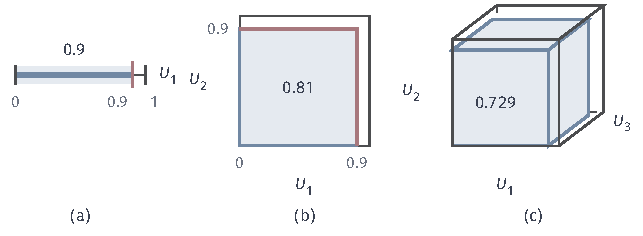
\includegraphics[width=109mm]{figures/07-probability/03-probability-limits/tikz/rvconv-error-event/figure.pdf}
 \caption{累计最大值的超差事件$\{1-M_n>0.1\}$。(a)$n=1$：线段$[0,0.9]$。(b)$n=2$：单位正方形中边长$0.9$的正方形，红线是事件的边界。(c)$n=3$：单位立方体中边长$0.9$的立方体。浅蓝区域的概率依次为$0.9$、$0.81$、$0.729$。}
 \label{fig:rvconv-error-event}
\end{BookInlineFigure}

\begin{definition}[依概率收敛]
\label{def:rvconv-in-probability}
若对每个$\varepsilon>0$，
\begin{equation}
 \lim_{n\to\infty}\mathbb{P}\bigl(\lvert X_n-X\rvert>\varepsilon\bigr)=0 ,
 \label{eq:rvconv-in-probability}
\end{equation}
称$X_n$\term{依概率收敛}（convergence in probability）到$X$，记作$X_n\xrightarrow{\mathbb{P}}X$。
\end{definition}

把“$>\varepsilon$”换成“$\geq\varepsilon$”得到同一个概念，因为两种事件互相夹住：
\[
 \{\lvert X_n-X\rvert>\varepsilon\}\subseteq\{\lvert X_n-X\rvert\geq\varepsilon\}\subseteq\{\lvert X_n-X\rvert>\varepsilon/2\} .
\]
由式~\eqref{eq:rvconv-max-tail}，$M_n\xrightarrow{\mathbb{P}}1$。依概率收敛就是卷四的依测度收敛，测度换成了概率。

\paragraph{移动区块}
依概率收敛只要求每一项的超差事件变小，并不要求它们停在同一个地方。下面的例子让超差事件在$\Omega$上来回移动。对$k=1,2,\dots$与$j=0,1,\dots,k-1$，令第$k$层第$j$段为$[j/k,(j+1)/k)$，按层从小到大、层内从左到右排成一列。第$n$项对应
\[
 n=\frac{k(k-1)}{2}+j+1,\qquad B_n=\mathbf{1}_{\{j/k\leq U<(j+1)/k\}} .
\]
前几项依次是$\mathbf{1}_{[0,1)}(U)$、$\mathbf{1}_{[0,1/2)}(U)$、$\mathbf{1}_{[1/2,1)}(U)$、$\mathbf{1}_{[0,1/3)}(U)$，等等。

对$0<\varepsilon<1$，第$n$项的超差事件就是$U$落在当前那一段，概率是段长$1/k$。$n$增大时层号$k$趋于无穷，所以
\[
 \mathbb{P}(\lvert B_n\rvert>\varepsilon)=\frac1k\to0,\qquad B_n\xrightarrow{\mathbb{P}}0 .
\]

但每一层的$k$段恰好铺满$[0,1)$，无论$U(\omega)$取什么值，每一层里都恰有一项等于$1$。所以对每一个$\omega$，数列$B_n(\omega)$中$1$出现无穷多次，$0$也出现无穷多次，它在任何一条记录上都不收敛。取$U(\omega)=0.37$，第$k$层里取值为$1$的是$j=\lfloor0.37k\rfloor$那一项，前几个序号是
\[
 n=1,\ 2,\ 5,\ 8,\ 12,\ 18,\ 24,\ 31,\ \dots
\]

\begin{BookInlineFigure}
 \centering
 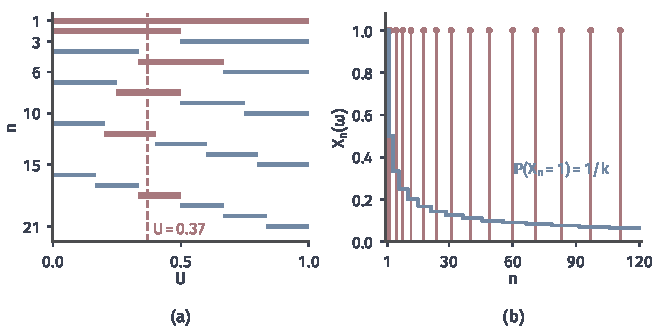
\includegraphics[width=112mm]{figures/07-probability/03-probability-limits/matplotlib/rvconv-blocks/figure.pdf}
 \caption{移动区块$B_n$。(a)前六层共$21$项：第$n$行的横条是$\{B_n=1\}$对应的$U$值区间，红色横条是被$U=0.37$穿过的那一项。(b)$U=0.37$这条记录上的$B_n(\omega)$，$n\leq120$：红色竖线标出取值为$1$的项；蓝色台阶是超差概率$\mathbb{P}(B_n=1)=1/k$。}
 \label{fig:rvconv-blocks}
\end{BookInlineFigure}

图~\ref{fig:rvconv-blocks}把两种读法放在一起。(a)中逐行看，每一行的横条越来越短，这是依概率收敛控制的量；沿红色虚线竖着看，就是一条记录，每一层都要碰到一个横条。(b)中蓝色台阶趋于零，红线却永不消失。大误差总会发生，只是发生在哪些记录上随$n$改变。

\paragraph{与几乎必然收敛对照}
两种收敛的差别在于控制的对象。依概率收敛逐次控制超差事件的大小，每个$n$单独检查；几乎必然收敛控制每条记录最终的行为，要求同一个$\omega$在某项之后再也不落入超差事件。前者是“在每一时刻，出问题的记录很少”，后者是“几乎每条记录，迟早不再出问题”。第~\ref{sec:rvconv-comparison}节证明后者推出前者，移动区块说明反过来不成立。

\paragraph{极限的唯一性与和的收敛}
依概率极限同样只在零概率事件上有差别。若$X_n\xrightarrow{\mathbb{P}}X$且$X_n\xrightarrow{\mathbb{P}}X'$，由三角不等式，$\lvert X-X'\rvert>2\varepsilon$时$\lvert X_n-X\rvert$与$\lvert X_n-X'\rvert$至少有一个大于$\varepsilon$，所以
\[
 \mathbb{P}\bigl(\lvert X-X'\rvert>2\varepsilon\bigr)\leq\mathbb{P}\bigl(\lvert X_n-X\rvert>\varepsilon\bigr)+\mathbb{P}\bigl(\lvert X_n-X'\rvert>\varepsilon\bigr).
\]
右边趋于零，左边与$n$无关，故为零。令$\varepsilon=1/k$并对$k$取可数并，得$\mathbb{P}(X\neq X')=0$。

同样的论证给出和的收敛：若$X_n\xrightarrow{\mathbb{P}}X$，$Y_n\xrightarrow{\mathbb{P}}Y$，则
\[
 \mathbb{P}\bigl(\lvert(X_n+Y_n)-(X+Y)\rvert>2\varepsilon\bigr)\leq\mathbb{P}\bigl(\lvert X_n-X\rvert>\varepsilon\bigr)+\mathbb{P}\bigl(\lvert Y_n-Y\rvert>\varepsilon\bigr)\to0 ,
\]
即$X_n+Y_n\xrightarrow{\mathbb{P}}X+Y$。两个超差事件各自很小，它们的并也很小，这种“并集上界”是处理依概率收敛的基本手段。

\subsection{\texorpdfstring{$L^{p}$}{Lp}收敛}
\label{sec:rvconv-lp}

超差概率只数大误差出现的机会，不管大误差有多大。另一种自然的要求是误差的平均大小趋于零。对$1\leq p<\infty$，误差绝对值的$p$次幂取期望，得到一个数$\mathbb{E}\bigl[\lvert X_n-X\rvert^{p}\bigr]$，大误差在其中按$p$次幂加权。

\begin{definition}[$L^{p}$收敛]
\label{def:rvconv-lp}
设$1\leq p<\infty$，$\mathbb{E}[\lvert X\rvert^{p}]<\infty$，且对每个$n$有$\mathbb{E}[\lvert X_n\rvert^{p}]<\infty$。若
\begin{equation}
 \lim_{n\to\infty}\mathbb{E}\bigl[\lvert X_n-X\rvert^{p}\bigr]=0 ,
 \label{eq:rvconv-lp}
\end{equation}
称$X_n$\term{$L^p$收敛}（convergence in $L^p$）到$X$，记作$X_n\xrightarrow{L^{p}}X$。
\end{definition}

矩有限的假设保证误差的$p$阶矩有意义。由$t\mapsto t^{p}$的凸性，对实数$a,b$有
\[
 \lvert a-b\rvert^{p}\leq2^{p-1}\bigl(\lvert a\rvert^{p}+\lvert b\rvert^{p}\bigr),
\]
所以$X_n$与$X$的$p$阶矩有限时，误差的$p$阶矩也有限。

把$p$阶矩开$p$次方，记
\[
 \lVert X\rVert_{p}=\bigl(\mathbb{E}[\lvert X\rvert^{p}]\bigr)^{1/p} ,
\]
它是卷四$L^{p}$范数在概率空间上的写法，$L^{p}$收敛就是$\lVert X_n-X\rVert_{p}\to0$。若同一列还$L^{p}$收敛到$X'$，由Minkowski不等式，
\[
 \lVert X-X'\rVert_{p}\leq\lVert X_n-X\rVert_{p}+\lVert X_n-X'\rVert_{p}\to0 ,
\]
左边与$n$无关，故为零，$X=X'$几乎必然。

\paragraph{平均绝对误差与均方误差}
$p=1$时，$\mathbb{E}[\lvert X_n-X\rvert]$是\emph{平均绝对误差}；$p=2$时，$\mathbb{E}[(X_n-X)^{2}]$是\emph{均方误差}，$L^{2}$收敛也称\term{均方收敛}（mean-square convergence）。目标是常数$c$时，均方误差可以拆成方差与偏差平方之和。在$X_n-c=(X_n-\mathbb{E}[X_n])+(\mathbb{E}[X_n]-c)$两边平方取期望，交叉项的期望为零，得到
\begin{equation}
 \mathbb{E}\bigl[(X_n-c)^{2}\bigr]=\operatorname{Var}(X_n)+\bigl(\mathbb{E}[X_n]-c\bigr)^{2} .
 \label{eq:rvconv-mse}
\end{equation}
所以$X_n\xrightarrow{L^{2}}c$当且仅当$\mathbb{E}[X_n]\to c$且$\operatorname{Var}(X_n)\to0$：均值要对准目标，波动要消失。

\paragraph{累计最大值的平均误差}
非负变量的矩可以由尾积分公式（第~\ref{chap:tail-probabilities}章）从生存函数算出：
\[
 \mathbb{E}[V^{p}]=\int_0^{\infty}p\,t^{p-1}\,\mathbb{P}(V>t)\,\mathrm{d}t .
\]
取$V=1-M_n$，它在$[0,1]$内取值，生存函数由式~\eqref{eq:rvconv-max-tail}给出。$p=1$时，
\[
 \mathbb{E}[1-M_n]=\int_0^{1}(1-t)^{n}\,\mathrm{d}t=\frac{1}{n+1} .
\]

$p=2$时，把$t=1-(1-t)$代入并分成两个积分，得到
\[
 \mathbb{E}\bigl[(1-M_n)^{2}\bigr]=2\int_0^{1}t(1-t)^{n}\,\mathrm{d}t=2\Bigl(\frac{1}{n+1}-\frac{1}{n+2}\Bigr)=\frac{2}{(n+1)(n+2)} .
\]
两者都趋于零，所以$M_n\xrightarrow{L^{1}}1$，$M_n\xrightarrow{L^{2}}1$。取$n=10$，平均绝对误差是$1/11\approx0.0909$，均方误差是$2/132\approx0.0152$。

用式~\eqref{eq:rvconv-mse}核对。偏差是$\mathbb{E}[M_{10}]-1=-1/11$，方差是均方误差减去偏差平方：
\[
 \operatorname{Var}(M_{10})=\frac{2}{132}-\frac{1}{121}\approx0.01515-0.00826=0.00689 .
\]
两部分大小相当：$M_n$总是低估$1$，平均低估$1/(n+1)$，同时围绕自己的均值波动。

\paragraph{稀有大值}
$L^{p}$收敛对大误差特别敏感。看$Z_n=\sqrt{n}\,\mathbf{1}_{\{U<1/n\}}$：它以概率$1/n$取$\sqrt n$，其余时候取$0$，所以
\begin{equation}
 \mathbb{E}\bigl[\lvert Z_n\rvert^{p}\bigr]=n^{p/2}\cdot\frac1n=n^{p/2-1} .
 \label{eq:rvconv-spike-moments}
\end{equation}
$p=1$时这是$n^{-1/2}\to0$，$p=2$时恒为$1$，$p=3$时是$n^{1/2}\to\infty$。同一列变量$L^{1}$收敛到$0$，却不$L^{2}$收敛。

把高度换成$n$，$Y_n=n\,\mathbf{1}_{\{U<1/n\}}$的平均绝对误差恒为$\mathbb{E}[Y_n]=1$，连$L^{1}$收敛也不成立。另一方面，$Y_n$与$Z_n$都在$U\geq1/n$时为零；对任何$U(\omega)>0$，$n>1/U(\omega)$以后两者都等于$0$，而$\mathbb{P}(U=0)=0$，所以它们都几乎必然收敛到$0$。超差概率是$1/n$，它们也依概率收敛到$0$。误差发生得越来越少，但每次发生时越来越大，平均误差能否消失取决于“少”与“大”谁占上风，而$p$越大，大误差的分量越重。

移动区块则相反：误差只取$0$和$1$，没有大值，$\mathbb{E}[\lvert B_n\rvert^{p}]=1/k\to0$，所以它在每个$L^{p}$中收敛到$0$，尽管在任何一条记录上都不收敛。

\paragraph{随机向量}
以上三种收敛对随机向量$\bm{X}_n,\bm{X}\in\mathbb{R}^{d}$同样适用，只需把$\lvert X_n-X\rvert$换成欧氏范数$\lVert\bm{X}_n-\bm{X}\rVert_2$。由于对每个分量$i$都有
\[
 \lvert x_i\rvert\leq\lVert\bm{x}\rVert_2\leq\lvert x_1\rvert+\dots+\lvert x_d\rvert ,
\]
向量的每一种收敛都等价于各个分量的同种收敛。维数固定时，只需研究实随机变量。


\section{收敛方式的比较}
\label{sec:rvconv-comparison}

三种收敛控制的对象不同：几乎必然收敛管每条记录的最终行为，依概率收敛管每一项超差事件的大小，$L^{p}$收敛管误差的平均大小。上一节的例子已经显示它们并不等价。哪些要求能推出另一些？推不出时，缺的是哪一种控制？

在一般测度空间上，几乎处处收敛推出依测度收敛需要总测度有限，$L^{r}$收敛推出较低阶的$L^{p}$收敛也需要总测度有限。概率空间的总质量为一，这两个条件自动满足，于是得到下面三条蕴含关系。

\begin{theorem}[收敛方式的蕴含关系]
\label{thm:rvconv-implications}
设$X_n,X$是同一概率空间上的实随机变量，$1\leq p<r<\infty$。
\begin{enumerate}
 \item 若$X_n\xrightarrow{\mathrm{a.s.}}X$，则$X_n\xrightarrow{\mathbb{P}}X$。
 \item 若$X_n\xrightarrow{L^{p}}X$，则$X_n\xrightarrow{\mathbb{P}}X$；更具体地，对每个$\varepsilon>0$，
 \begin{equation}
  \mathbb{P}\bigl(\lvert X_n-X\rvert>\varepsilon\bigr)\leq\frac{\mathbb{E}\bigl[\lvert X_n-X\rvert^{p}\bigr]}{\varepsilon^{p}} .
  \label{eq:rvconv-markov-lp}
 \end{equation}
 \item 若$X_n\xrightarrow{L^{r}}X$，则$X_n\xrightarrow{L^{p}}X$；更具体地，
 \begin{equation}
  \lVert X_n-X\rVert_{p}\leq\lVert X_n-X\rVert_{r} .
  \label{eq:rvconv-lp-monotone}
 \end{equation}
\end{enumerate}
\end{theorem}

\begin{proof}
第1条。固定$\varepsilon>0$，令
\[
 G_N=\bigcup_{n\geq N}\bigl\{\lvert X_n-X\rvert>\varepsilon\bigr\},
\]
即从第$N$项起至少超差一次的记录。$G_N$随$N$递减。若$\omega$属于每一个$G_N$，则$\omega$上超差发生无穷多次，$X_n(\omega)\not\to X(\omega)$；所以$\bigcap_NG_N\subseteq\{X_n\not\to X\}$，它的概率为零。

概率测度对递减事件列连续（第~\ref{chap:probability-spaces}章），这里用到总质量有限：
\[
 \mathbb{P}(G_N)\to\mathbb{P}\Bigl(\bigcap_NG_N\Bigr)=0 .
\]
而第$N$项的超差事件含于$G_N$，它的概率不超过$\mathbb{P}(G_N)$，也趋于零。

第2条。超差事件含于$p$次幂的超差事件：
\[
 \{\lvert X_n-X\rvert>\varepsilon\}\subseteq\{\lvert X_n-X\rvert^{p}\geq\varepsilon^{p}\} .
\]
对非负随机变量$\lvert X_n-X\rvert^{p}$和阈值$\varepsilon^{p}$用Markov不等式（第~\ref{chap:tail-probabilities}章），即得式~\eqref{eq:rvconv-markov-lp}。右边趋于零，左边也趋于零。

第3条。第~\ref{chap:random-variable-moments}章由Jensen不等式证明了绝对矩开相应次方后随阶数单调增加：对任意随机变量$V$，
\[
 \bigl(\mathbb{E}[\lvert V\rvert^{p}]\bigr)^{1/p}\leq\bigl(\mathbb{E}[\lvert V\rvert^{r}]\bigr)^{1/r} .
\]
取$V=X_n-X$即得式~\eqref{eq:rvconv-lp-monotone}。
\end{proof}

第1条证明中的$G_N$把整个尾段的超差合在一起。几乎必然收敛控制的正是这个尾段的并，依概率收敛只控制其中一项，前者自然更强；第~\ref{sec:rvconv-infinitely-often}小节会把这一观察写成等价条件。第3条在一般测度空间上要多出一个因子，即总测度的$1/p-1/r$次幂，概率空间中这个因子是$1$。

\paragraph{用累计最大值核对}
取$n=10$，$\varepsilon=0.1$。精确的超差概率是$0.9^{10}\approx0.349$。由式~\eqref{eq:rvconv-markov-lp}，用平均绝对误差$1/11$与均方误差$2/132$分别得到上界
\[
 \frac{1/11}{0.1}\approx0.909,\qquad \frac{2/132}{0.01}\approx1.52 .
\]
两个界都成立，后者大于$1$而没有信息。式~\eqref{eq:rvconv-lp-monotone}也可以直接核对：
\[
 \lVert1-M_{10}\rVert_{1}\approx0.0909\leq\lVert1-M_{10}\rVert_{2}=\sqrt{2/132}\approx0.123 .
\]

\paragraph{逆命题的反例}
三条蕴含关系都不能反过来。表~\ref{tab:rvconv-examples}汇总了贯穿例子的收敛情况，其中独立示性变量$\xi_n$取$p_n=1/n$，它不几乎必然收敛这一点要到第~\ref{sec:rvconv-borel-cantelli}小节才能证明。

\begin{BookInlineTable}
 \centering
 \begin{tabular}{@{}lcccc@{}}
  \toprule
  随机变量列 & 几乎必然 & 依概率 & $L^{1}$ & $L^{2}$ \\
  \midrule
  $M_n\to1$ & 是 & 是 & 是 & 是 \\
  移动区块$B_n\to0$ & 否 & 是 & 是 & 是 \\
  $\xi_n\to0$，$p_n=1/n$ & 否 & 是 & 是 & 是 \\
  $Z_n=\sqrt n\,\mathbf{1}_{\{U<1/n\}}\to0$ & 是 & 是 & 是 & 否 \\
  $Y_n=n\,\mathbf{1}_{\{U<1/n\}}\to0$ & 是 & 是 & 否 & 否 \\
  \bottomrule
 \end{tabular}
 \caption{贯穿例子在四种意义下是否收敛。}
 \label{tab:rvconv-examples}
\end{BookInlineTable}

表中的“否”来自两种不同的缺陷。第一种是缺少尾部控制：$Y_n$和$Z_n$的超差概率$1/n$趋于零，每条记录最终也归于零，但偶尔出现的误差越来越大，大到足以维持平均。依概率收敛与几乎必然收敛都只看误差是否超过$\varepsilon$，对超出多少一无所知，所以推不出$L^{p}$收敛。

第二种是缺少整列的逐样本控制：$B_n$和$\xi_n$的误差只取$0$或$1$，平均误差和超差概率一起趋于零，但超差事件在$\Omega$上不断移动或独立地重新出现，每条记录（或几乎每条记录）上都无穷多次超差。$L^{p}$收敛与依概率收敛都是逐项的要求，管不到同一条记录在不同时刻的表现，所以推不出几乎必然收敛。

\begin{BookInlineFigure}
 \centering
 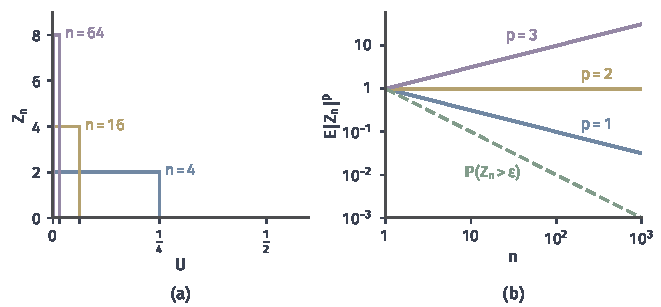
\includegraphics[width=112mm]{figures/07-probability/03-probability-limits/matplotlib/rvconv-power-spikes/figure.pdf}
 \caption{稀有大值$Z_n=\sqrt n\,\mathbf{1}_{\{U<1/n\}}$。(a)$Z_n$作为$U$的函数，$n=4,16,64$：高为$\sqrt n$、宽为$1/n$的矩形。(b)双对数坐标下的精确矩$\mathbb{E}[\lvert Z_n\rvert^{p}]=n^{p/2-1}$，$p=1,2,3$（蓝、黄、紫），绿色虚线是超差概率$1/n$（$0<\varepsilon<1$）。}
 \label{fig:rvconv-power-spikes}
\end{BookInlineFigure}

图~\ref{fig:rvconv-power-spikes}把第一种缺陷画出来。(a)中矩形越来越窄、越来越高；$p$阶矩是$\lvert Z_n\rvert^{p}$下方的面积，宽度按$1/n$缩小，高度的$p$次幂按$n^{p/2}$增长。(b)中各条直线的斜率$p/2-1$表明两者谁占上风：$p<2$时宽度胜出，$p=2$时恰好持平，$p>2$时高度胜出。超差概率的斜率是$-1$，它对高度完全不敏感。

\paragraph{较高阶与较低阶}
$Z_n$还说明第3条不能反过来：$L^{1}$收敛推不出$L^{2}$收敛。较低阶的平均把大误差压得较轻，较高阶的平均把它放得较重，所以控制高阶误差的要求更强。

\paragraph{两种收敛同时成立时}
若同一列变量既几乎必然收敛到$X$，又$L^{p}$收敛到$X'$，则由定理~\ref{thm:rvconv-implications}，两者都推出依概率收敛，再由依概率极限的唯一性，$X=X'$几乎必然。不同的收敛方式可能有的成立、有的不成立，但只要成立，极限就相同。

缺陷既然分成两种，就可以分别去补。超差事件如何才能只在每条记录上出现有限次？这是下一节的问题，答案依赖超差概率加起来是否有限，以及各事件是否独立。什么样的尾部条件能阻止稀有大值维持平均？这是第~\ref{sec:rvconv-expectation-limits}节的问题。


\section{几乎必然收敛的判别}
\label{sec:rvconv-as-criteria}

怎样判断一列随机变量是否几乎必然收敛？定义要求几乎每条记录上的数列收敛，直接检查每条记录通常做不到。本节把问题翻译成事件的语言：误差最终小于$\varepsilon$，就是超差事件从某项起不再发生，也就是它只发生有限次。于是问题变成：一列事件在几乎每条记录上是否只发生有限次？

\subsection{无穷多次发生的事件}
\label{sec:rvconv-infinitely-often}

给定事件列$A_1,A_2,\dots$。一条记录$\omega$可能落在其中无穷多个事件里，也可能只落在有限个里。图~\ref{fig:rvconv-limsup-grid}画了四条记录：$\omega_1$落在所有偶数号事件里，$\omega_3$落在平方数号事件里，都是无穷多次；$\omega_2$只落在四个事件里；$\omega_4$从不落入。

\begin{BookInlineFigure}
 \centering
 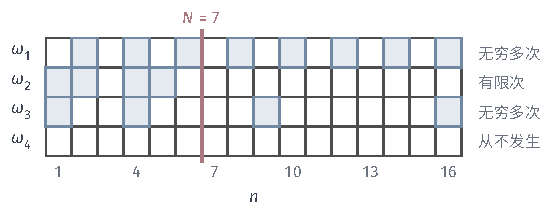
\includegraphics[width=94mm]{figures/07-probability/03-probability-limits/tikz/rvconv-limsup-grid/figure.pdf}
 \caption{事件的无穷次发生。每行是一条记录，第$n$列的浅蓝格表示该记录属于$A_n$。红线右侧是从$N=7$起的尾段：$\omega_1$与$\omega_3$在尾段中仍然出现，属于$\bigcup_{n\geq7}A_n$；$\omega_2$与$\omega_4$不属于。无论$N$取多大，$\omega_1$与$\omega_3$总留在尾段的并里。}
 \label{fig:rvconv-limsup-grid}
\end{BookInlineFigure}

“无穷多次”可以用可数次集合运算写出来。$\omega$落在无穷多个$A_n$中，等价于无论从哪一项$N$开始往后看，它都至少还落在一个$A_n$（$n\geq N$）中，即对每个$N$都有$\omega\in\bigcup_{n\geq N}A_n$。

\begin{definition}[事件的上极限与下极限]
\label{def:rvconv-limsup}
对事件列$(A_n)$，令
\begin{equation}
 \limsup_{n\to\infty}A_n=\bigcap_{N=1}^{\infty}\bigcup_{n\geq N}A_n,\qquad
 \liminf_{n\to\infty}A_n=\bigcup_{N=1}^{\infty}\bigcap_{n\geq N}A_n .
 \label{eq:rvconv-limsup}
\end{equation}
前者是$A_n$\term{无穷多次发生}（occurring infinitely often）的事件，也记作$\{A_n\ \text{i.o.}\}$；后者是从某项起$A_n$每次都发生的事件。
\end{definition}

两者都由可数次并与交得到，所以都是事件。取补集并交换并与交，得到
\[
 \Bigl(\limsup_{n\to\infty}A_n\Bigr)^{\mathrm{c}}=\bigcup_{N=1}^{\infty}\bigcap_{n\geq N}A_n^{\mathrm{c}}=\liminf_{n\to\infty}A_n^{\mathrm{c}} .
\]
右边说的是“存在$N$，从第$N$项起$A_n$不再发生”，也就是$A_n$只发生有限次。“无穷多次发生”与“最终不再发生”恰好互补。

尾段的并$\bigcup_{n\geq N}A_n$随$N$递减，由概率的连续性，
\begin{equation}
 \mathbb{P}\Bigl(\limsup_{n\to\infty}A_n\Bigr)=\lim_{N\to\infty}\mathbb{P}\Bigl(\bigcup_{n\geq N}A_n\Bigr) .
 \label{eq:rvconv-limsup-continuity}
\end{equation}
无穷多次发生的概率，就是“从第$N$项起至少再发生一次”的概率在$N\to\infty$时的极限。

\paragraph{应用于超差事件}
现在把$A_n$取为超差事件。对$\varepsilon>0$，记
\[
 A_n(\varepsilon)=\bigl\{\lvert X_n-X\rvert>\varepsilon\bigr\}.
\]
$\omega$上的数列$X_n(\omega)$收敛到$X(\omega)$，就是对每个$\varepsilon>0$，$\omega$只落在有限个$A_n(\varepsilon)$中。阈值有不可数多个，但$\varepsilon$越小超差事件越大，所以只需检查一列趋于零的阈值，例如$\varepsilon=1/k$。

\begin{theorem}[几乎必然收敛的事件判据]
\label{thm:rvconv-as-io}
以下三条等价：
\begin{enumerate}
 \item $X_n\xrightarrow{\mathrm{a.s.}}X$；
 \item 对每个$\varepsilon>0$，$\mathbb{P}\bigl(\limsup_nA_n(\varepsilon)\bigr)=0$；
 \item 对每个$\varepsilon>0$，
 \begin{equation}
  \lim_{N\to\infty}\mathbb{P}\Bigl(\sup_{n\geq N}\lvert X_n-X\rvert>\varepsilon\Bigr)=0 .
  \label{eq:rvconv-as-sup}
 \end{equation}
\end{enumerate}
并且在第2条中只需对$\varepsilon=1/k$（$k=1,2,\dots$）检查。
\end{theorem}

\begin{proof}
先写出不收敛的记录。$X_n(\omega)\not\to X(\omega)$当且仅当存在某个$k$，使$\lvert X_n(\omega)-X(\omega)\rvert>1/k$对无穷多个$n$成立。所以
\[
 \{X_n\not\to X\}=\bigcup_{k=1}^{\infty}\limsup_{n\to\infty}A_n(1/k) .
\]
右边是可数个事件的并，因此收敛集合是事件，这也补上了定义~\ref{def:rvconv-almost-sure}中可测性的说明。

1推2。对任意$\varepsilon>0$，取$k$使$1/k<\varepsilon$，则$A_n(\varepsilon)\subseteq A_n(1/k)$，于是$\limsup_nA_n(\varepsilon)$含于$\{X_n\not\to X\}$，概率为零。

2推1。只用$\varepsilon=1/k$：由上面的等式与可数次可加性，
\[
 \mathbb{P}(X_n\not\to X)\leq\sum_{k=1}^{\infty}\mathbb{P}\Bigl(\limsup_{n\to\infty}A_n(1/k)\Bigr)=0 .
\]

2与3等价。$\sup_{n\geq N}\lvert X_n-X\rvert>\varepsilon$当且仅当某个$n\geq N$使$\lvert X_n-X\rvert>\varepsilon$，所以
\[
 \Bigl\{\sup_{n\geq N}\lvert X_n-X\rvert>\varepsilon\Bigr\}=\bigcup_{n\geq N}A_n(\varepsilon) .
\]
由式~\eqref{eq:rvconv-limsup-continuity}，这个概率的极限就是$\mathbb{P}(\limsup_nA_n(\varepsilon))$。
\end{proof}

如果直接对所有$\varepsilon>0$取并，会得到不可数个事件的并，概率论不允许对它用可加性。单调性让我们只取可数个阈值，这是“阈值只需取一列趋于零的正有理数”的原因。

\paragraph{对照依概率收敛}
式~\eqref{eq:rvconv-as-sup}与依概率收敛的式~\eqref{eq:rvconv-in-probability}只差一个上确界：依概率收敛要求第$N$项的误差超标的概率趋于零，几乎必然收敛要求从第$N$项起的最大误差超标的概率趋于零。后者控制整个尾段，这再次说明它更强。

当误差的绝对值随$n$单调不增时，尾段的最大误差就是第$N$项的误差，两种收敛等价。累计最大值正是如此：$1-M_n$递减，超差事件随$n$缩小，尾段的并就是$A_N(\varepsilon)$。由式~\eqref{eq:rvconv-max-tail}，
\[
 \mathbb{P}\Bigl(\sup_{n\geq N}(1-M_n)>\varepsilon\Bigr)=(1-\varepsilon)^{N}\to0 ,
\]
这与第~\ref{sec:rvconv-almost-sure}小节的直接论证一致。移动区块则相反：每一层都铺满$[0,1)$，对$0<\varepsilon<1$和每个$N$，$\bigcup_{n\geq N}A_n(\varepsilon)=\Omega$，尾段并的概率恒为$1$。

\subsection{Borel–Cantelli引理}
\label{sec:rvconv-borel-cantelli}

上一小节把几乎必然收敛归结为$\mathbb{P}(\limsup_nA_n)=0$。尾段的并通常没有简单公式，但每个$A_n$的概率往往容易算。能否只用这些单项概率作出判断？答案取决于$\sum_n\mathbb{P}(A_n)$是否有限：有限时，用并集上界即可；无限时，还需要独立性。

\paragraph{概率可和的情形}
若各事件的概率之和有限，尾段的概率之和趋于零，尾段的并也就越来越不可能发生。

\begin{lemma}[Borel–Cantelli引理]
\label{lem:rvconv-borel-cantelli}
若事件列$(A_n)$满足$\sum_{n=1}^{\infty}\mathbb{P}(A_n)<\infty$，则
\begin{equation}
 \mathbb{P}\Bigl(\limsup_{n\to\infty}A_n\Bigr)=0 .
 \label{eq:rvconv-bc1}
\end{equation}
\end{lemma}

\begin{proof}
对每个$N$，$\limsup_nA_n\subseteq\bigcup_{n\geq N}A_n$。由可数次可加性给出的并集上界，
\[
 \mathbb{P}\Bigl(\limsup_{n\to\infty}A_n\Bigr)\leq\mathbb{P}\Bigl(\bigcup_{n\geq N}A_n\Bigr)\leq\sum_{n\geq N}\mathbb{P}(A_n) .
\]
右边是收敛级数的尾和，$N\to\infty$时趋于零，左边与$N$无关，所以为零。
\end{proof}

这个结论称为\term{Borel–Cantelli引理}（Borel–Cantelli lemma）。证明只用了并集上界，没有用到事件之间的任何关系，所以它不要求独立。级数收敛的直观含义是事件发生的平均次数有限：第~\ref{sec:rvconv-monotone}小节会证明发生次数$\sum_n\mathbf{1}_{A_n}$的期望等于$\sum_n\mathbb{P}(A_n)$，平均次数有限的计数几乎必然有限。

\paragraph{独立示性变量：概率可和}
回到独立示性变量$\xi_n=\mathbf{1}_{\{U_n<p_n\}}$，取$p_n=1/n^{2}$。级数
\[
 \sum_{n=1}^{\infty}\frac{1}{n^{2}}=\frac{\pi^{2}}{6}\approx1.645
\]
收敛，由引理~\ref{lem:rvconv-borel-cantelli}，几乎每条记录上只有有限个$\xi_n=1$。对这样的记录，从某项起$\xi_n=0$，所以$\xi_n\xrightarrow{\mathrm{a.s.}}0$。

这里的事件恰好独立，尾段并的概率也能精确算出。由独立性和补事件，对$N\geq2$，
\[
 \mathbb{P}\Bigl(\bigcup_{n=N}^{M}A_n\Bigr)=1-\prod_{n=N}^{M}\Bigl(1-\frac{1}{n^{2}}\Bigr)=1-\prod_{n=N}^{M}\frac{(n-1)(n+1)}{n\cdot n} .
\]

乘积是裂项的：分子中的$n-1$与前一项分母的$n$相消，$n+1$与后一项分母的$n$相消，只剩下首尾两个因子，
\[
 \prod_{n=N}^{M}\frac{(n-1)(n+1)}{n\cdot n}=\frac{N-1}{N}\cdot\frac{M+1}{M} .
\]
令$M\to\infty$，得到$\mathbb{P}\bigl(\bigcup_{n\geq N}A_n\bigr)=1/N$。$N=10$时它等于$0.1$，并集上界$\sum_{n\geq10}n^{-2}\approx0.105$，两者相当接近，见图~\ref{fig:rvconv-bc-unions}(a)。

\paragraph{概率不可和的情形}
级数发散时，并集上界失效。此时事件是否无穷多次发生取决于事件之间的关系。若各事件独立，发散的级数迫使它们无穷多次发生。

\begin{lemma}[独立事件的Borel–Cantelli引理]
\label{lem:rvconv-borel-cantelli-2}
若事件$A_1,A_2,\dots$相互独立，且$\sum_{n=1}^{\infty}\mathbb{P}(A_n)=\infty$，则
\begin{equation}
 \mathbb{P}\Bigl(\limsup_{n\to\infty}A_n\Bigr)=1 .
 \label{eq:rvconv-bc2}
\end{equation}
\end{lemma}

\begin{proof}
只需证明补事件的概率为零。由上一小节，补事件是
\[
 \Bigl(\limsup_{n\to\infty}A_n\Bigr)^{\mathrm{c}}=\bigcup_{N=1}^{\infty}\bigcap_{n\geq N}A_n^{\mathrm{c}} ,
\]
它是可数个事件的并，所以只需证明对每个$N$，
\[
 \mathbb{P}\Bigl(\bigcap_{n\geq N}A_n^{\mathrm{c}}\Bigr)=0 .
\]

相互独立事件的补事件仍相互独立。对$M\geq N$，记$p_n=\mathbb{P}(A_n)$，再用$1-x\leq\mathrm{e}^{-x}$（$x\in\mathbb{R}$），得到
\[
 \mathbb{P}\Bigl(\bigcap_{n=N}^{M}A_n^{\mathrm{c}}\Bigr)=\prod_{n=N}^{M}(1-p_n)\leq\exp\Bigl(-\sum_{n=N}^{M}p_n\Bigr) .
\]
级数发散，所以对固定的$N$，$\sum_{n=N}^{M}p_n\to\infty$（$M\to\infty$），右边趋于零。

$\bigcap_{n=N}^{M}A_n^{\mathrm{c}}$随$M$递减到$\bigcap_{n\geq N}A_n^{\mathrm{c}}$，由概率的连续性，后者的概率是左边的极限，等于零。
\end{proof}

不等式$1-x\leq\mathrm{e}^{-x}$把乘积化为和的指数：每个独立事件都有一份“不发生”的概率，它们相乘以后被发散的级数压到零。独立性用在第一个等号上，把交的概率写成乘积。

\paragraph{独立示性变量：概率不可和}
取$p_n=1/n$。$\sum_n1/n=\infty$，事件又相互独立，由引理~\ref{lem:rvconv-borel-cantelli-2}，几乎每条记录上都有无穷多个$\xi_n=1$，所以$\xi_n$几乎必然不收敛到$0$。另一方面，$\mathbb{P}(\xi_n=1)=1/n\to0$，$\mathbb{E}[\xi_n^{p}]=1/n\to0$，它依概率收敛、在每个$L^{p}$中收敛到$0$。这就补上了表~\ref{tab:rvconv-examples}中的第三行。

尾段并的概率同样可以精确计算。对$N\geq2$，乘积仍然裂项：
\[
 \mathbb{P}\Bigl(\bigcup_{n=N}^{M}A_n\Bigr)=1-\prod_{n=N}^{M}\frac{n-1}{n}=1-\frac{N-1}{M} .
\]
无论$N$多大，令$M\to\infty$它都趋于$1$。取$N=10$，$M=100$时已是$0.91$。图~\ref{fig:rvconv-bc-unions}(b)画出$N=10,100,1000$三条曲线：起点越晚，需要等得越久，但最终都要发生。

\begin{BookInlineFigure}
 \centering
 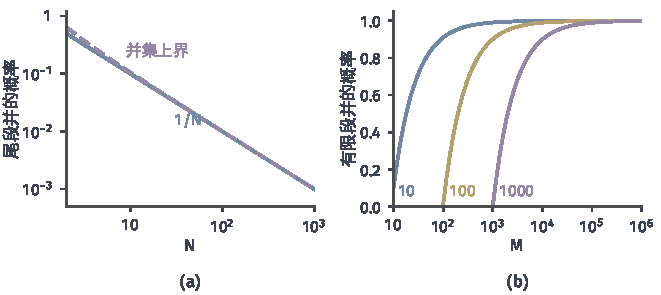
\includegraphics[width=112mm]{figures/07-probability/03-probability-limits/matplotlib/rvconv-bc-unions/figure.pdf}
 \caption{独立事件$A_n$尾段并的精确概率。(a)$\mathbb{P}(A_n)=1/n^{2}$：$\mathbb{P}(\bigcup_{n\geq N}A_n)=1/N$（蓝线）与并集上界$\sum_{n\geq N}n^{-2}$（紫色虚线），双对数坐标。(b)$\mathbb{P}(A_n)=1/n$：$\mathbb{P}(\bigcup_{n=N}^{M}A_n)=1-(N-1)/M$随$M$的变化，曲线旁的数字是起点$N$。}
 \label{fig:rvconv-bc-unions}
\end{BookInlineFigure}

图~\ref{fig:rvconv-bern-paths}从样本记录的角度看同一件事，画的是前$n$项中发生的次数$C_n=\sum_{k\leq n}\xi_k$。$p_n=1/n$时，计数在对数横轴上持续上升，期望是调和数$H_n\approx\ln n+0.577$，没有上限。$p_n=1/n^{2}$时，计数很早就停住，$10^{5}$项里只发生一两次。

\begin{BookInlineFigure}
 \centering
 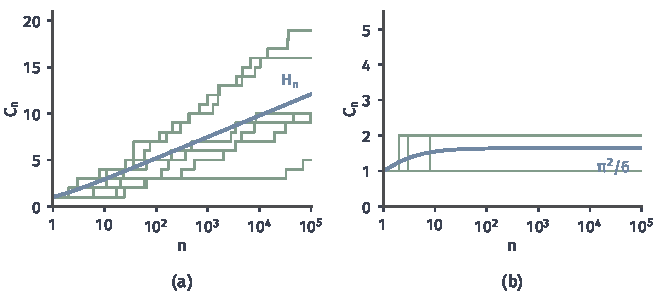
\includegraphics[width=112mm]{figures/07-probability/03-probability-limits/matplotlib/rvconv-bern-paths/figure.pdf}
 \caption{独立示性变量的累计发生次数$C_n=\sum_{k\leq n}\xi_k$，六条模拟记录（绿色，种子$2026$），横轴为对数刻度，$n\leq10^{5}$。蓝线是期望$\mathbb{E}[C_n]=\sum_{k\leq n}p_k$。(a)$p_n=1/n$，期望为调和数$H_n$，趋于无穷。(b)$p_n=1/n^{2}$，期望趋于$\pi^{2}/6\approx1.645$。}
 \label{fig:rvconv-bern-paths}
\end{BookInlineFigure}

两个引理合起来，对独立示性变量给出完整的回答：$\xi_n\xrightarrow{\mathrm{a.s.}}0$当且仅当$\sum_np_n<\infty$，而$\xi_n\xrightarrow{\mathbb{P}}0$当且仅当$p_n\to0$。$p_n\to0$但$\sum_np_n=\infty$的情形，例如$p_n=1/n$或$1/\sqrt{n}$，正好落在两者之间。它们还说明，独立事件的无穷多次发生只有两种可能：概率为$0$或为$1$。

\paragraph{去掉独立条件}
第二个引理的独立条件不能省略。取同一个事件重复：$A_n=A$对一切$n$成立，其中$0<\mathbb{P}(A)<1$。这时$\sum_n\mathbb{P}(A_n)=\infty$，但
\[
 \limsup_{n\to\infty}A_n=A,\qquad \mathbb{P}\Bigl(\limsup_{n\to\infty}A_n\Bigr)=\mathbb{P}(A)\in(0,1) .
\]
各项完全相关：在$A$上每次都发生，在$A$外从不发生。

依赖还可以把概率压到零。取$A_n=\{U<1/n\}$，$\sum_n1/n=\infty$，但这些事件递减，
\[
 \limsup_{n\to\infty}A_n=\bigcap_{n}\{U<1/n\}=\{U\leq0\},
\]
它的概率为零。所以概率发散时，没有独立性就什么也推不出：无穷多次发生的概率可以是$0$与$1$之间的任何值。第一个引理则对任何依赖结构都成立，这是两个方向在条件上的根本不对称。

\subsection{子列刻画}
\label{sec:rvconv-subsequence}

依概率收敛推不出几乎必然收敛，缺的是对整列的控制。但如果只看一部分项，跳过中间的项，超差概率就可能加起来有限。这是本小节的出发点：从依概率收敛的列中总能挑出几乎必然收敛的子列。

\begin{theorem}[几乎必然收敛的子列]
\label{thm:rvconv-subsequence}
若$X_n\xrightarrow{\mathbb{P}}X$，则存在子列$n_1<n_2<\cdots$，使$X_{n_k}\xrightarrow{\mathrm{a.s.}}X$。
\end{theorem}

\begin{proof}
由依概率收敛，对每个$k$，存在$N_k$使$n\geq N_k$时$\mathbb{P}(\lvert X_n-X\rvert>2^{-k})\leq2^{-k}$。递归地取$n_k\geq N_k$且$n_k>n_{k-1}$，令
\[
 E_k=\bigl\{\lvert X_{n_k}-X\rvert>2^{-k}\bigr\},\qquad \mathbb{P}(E_k)\leq2^{-k} .
\]

$\sum_k2^{-k}=1<\infty$，由引理~\ref{lem:rvconv-borel-cantelli}，$\mathbb{P}(\limsup_kE_k)=0$。对不在这个零概率事件中的$\omega$，存在$K(\omega)$，使$k\geq K(\omega)$时$\omega\notin E_k$，即
\[
 \lvert X_{n_k}(\omega)-X(\omega)\rvert\leq2^{-k},\qquad k\geq K(\omega) .
\]
右边趋于零，所以$X_{n_k}(\omega)\to X(\omega)$。
\end{proof}

阈值$2^{-k}$随$k$缩小，所以一个零概率例外集就同时照顾了所有精度，不需要再对$\varepsilon$取并。挑选子列的作用是让超差概率快速下降到可以求和，原列的超差概率可能下降得太慢。

\paragraph{移动区块的子列}
$B_n$依概率收敛到$0$，按定理应有几乎必然收敛的子列。每层取第一段即可：$n_k=k(k-1)/2+1$，
\[
 B_{n_k}=\mathbf{1}_{\{U<1/k\}} .
\]
对$U(\omega)>0$，$k>1/U(\omega)$以后$B_{n_k}(\omega)=0$，所以$B_{n_k}\xrightarrow{\mathrm{a.s.}}0$。图~\ref{fig:rvconv-subsequence}画出两条记录：原列在每层都碰到一次$1$，子列从某层起恒为零，而“某层”随记录改变。

\begin{BookInlineFigure}
 \centering
 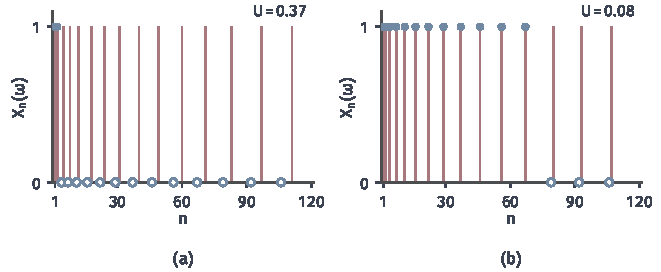
\includegraphics[width=112mm]{figures/07-probability/03-probability-limits/matplotlib/rvconv-subsequence/figure.pdf}
 \caption{移动区块的几乎必然收敛子列。红色竖线是原列$B_n(\omega)$取$1$的项，$n\leq120$；蓝点是子列$B_{n_k}=\mathbf{1}_{\{U<1/k\}}$（每层第一段）的取值，实心为$1$，空心为$0$。(a)$U=0.37$：子列只在$k=1,2$取$1$。(b)$U=0.08$：子列在$k\leq12$取$1$，此后恒为$0$。}
 \label{fig:rvconv-subsequence}
\end{BookInlineFigure}

这个子列的超差概率$1/k$加起来是发散的，它却几乎必然收敛：事件$\{U<1/k\}$递减，不独立。Borel–Cantelli引理是充分条件而不是必要条件。若按定理证明的办法挑选，会取到$k=2^{m}$那些层的第一段，超差概率$2^{-m}$可以求和。

\paragraph{独立示性变量的子列}
$p_n=1/n$时整列$\xi_n$不几乎必然收敛，但子列$n_k=k^{2}$的超差概率是$1/k^{2}$，可以求和。由引理~\ref{lem:rvconv-borel-cantelli}，$\xi_{k^{2}}\xrightarrow{\mathrm{a.s.}}0$。整列在几乎每条记录上无穷多次取$1$，但这些$1$几乎都落在跳过的项上。

\paragraph{完整的刻画}
一个几乎必然收敛的子列只是依概率收敛的一个推论，不足以反推整列依概率收敛。例如$X_{2m}=0$，$X_{2m-1}=\mathbf{1}_{\{U<1/2\}}$：偶数项的子列恒为零，而奇数项的超差概率恒为$1/2$，整列不依概率收敛到$0$。要刻画依概率收敛，必须对每一个子列都提出要求。

\begin{theorem}[依概率收敛的子列刻画]
\label{thm:rvconv-subsequence-criterion}
$X_n\xrightarrow{\mathbb{P}}X$当且仅当：对$(X_n)$的每个子列$(X_{n_k})$，都存在进一步的子列$(X_{n_{k_j}})$，使$X_{n_{k_j}}\xrightarrow{\mathrm{a.s.}}X$。
\end{theorem}

\begin{proof}
必要性。依概率收敛列的每个子列仍依概率收敛到$X$，对这个子列用定理~\ref{thm:rvconv-subsequence}即可。

充分性用反证法。若$X_n$不依概率收敛到$X$，则存在$\varepsilon>0$、$\delta>0$和子列$(n_k)$，使
\[
 \mathbb{P}\bigl(\lvert X_{n_k}-X\rvert>\varepsilon\bigr)\geq\delta,\qquad k=1,2,\dots
\]
按假设，它有进一步的子列几乎必然收敛到$X$，由定理~\ref{thm:rvconv-implications}也依概率收敛到$X$，其超差概率趋于零，与上式矛盾。
\end{proof}

前一个例子中，奇数项组成的子列没有任何进一步的子列收敛到$0$，所以条件不满足，这与整列不收敛一致。

\paragraph{几乎必然收敛没有这样的刻画}
移动区块满足定理~\ref{thm:rvconv-subsequence-criterion}中的条件：每个子列仍依概率收敛到$0$，因而有几乎必然收敛的进一步子列。但整列不几乎必然收敛。所以“每个子列都有收敛到$X$的进一步子列”这一条件，对几乎必然收敛不是充分的。

对由拓扑或距离定义的收敛，这一条件总是充分的：若$x_n\not\to x$，就有$x$的一个邻域和一个整个落在邻域外的子列，这个子列的任何进一步子列都不收敛到$x$。因此不存在一种距离，使随机变量按这种距离收敛恰好是几乎必然收敛。

依概率收敛则可以用一个平均量描述。对$0<\varepsilon\leq1$，把误差在$\varepsilon$处分开，并分别用$\min\{\lvert x\rvert,1\}\leq\varepsilon$（当$\lvert x\rvert\leq\varepsilon$）与$\min\{\lvert x\rvert,1\}\leq1$估计，再对超差事件用Markov不等式，得到
\[
 \varepsilon\,\mathbb{P}\bigl(\lvert X_n-X\rvert>\varepsilon\bigr)\leq\mathbb{E}\bigl[\min\{\lvert X_n-X\rvert,1\}\bigr]\leq\varepsilon+\mathbb{P}\bigl(\lvert X_n-X\rvert>\varepsilon\bigr) .
\]
所以$X_n\xrightarrow{\mathbb{P}}X$当且仅当$\mathbb{E}[\min\{\lvert X_n-X\rvert,1\}]\to0$。截去大于$1$的部分，是为了让稀有大值不影响这个平均，它衡量的只是“超差的机会”。

\paragraph{连续映射}
子列刻画的一个直接用途是传递依概率收敛。设$g:\mathbb{R}\to\mathbb{R}$连续，$X_n\xrightarrow{\mathbb{P}}X$，要证$g(X_n)\xrightarrow{\mathbb{P}}g(X)$。直接估计$\mathbb{P}(\lvert g(X_n)-g(X)\rvert>\varepsilon)$需要$g$的一致连续性，而$g$在整条实轴上未必一致连续。

用子列刻画则只需逐点的连续性。任取一个子列，它有进一步的子列几乎必然收敛到$X$；在这个子列上，对收敛的记录$\omega$，由$g$的连续性，$g(X_{n_{k_j}}(\omega))\to g(X(\omega))$，即$g(X_{n_{k_j}})\xrightarrow{\mathrm{a.s.}}g(X)$。由定理~\ref{thm:rvconv-subsequence-criterion}，$g(X_n)\xrightarrow{\mathbb{P}}g(X)$。例如$X_n\xrightarrow{\mathbb{P}}X$推出$X_n^{2}\xrightarrow{\mathbb{P}}X^{2}$。


\section{期望与极限}
\label{sec:rvconv-expectation-limits}

$Y_n=n\,\mathbf{1}_{\{U<1/n\}}$几乎必然收敛到$0$，期望却恒为$1$：
\[
 \lim_{n\to\infty}\mathbb{E}[Y_n]=1\neq0=\mathbb{E}\Bigl[\lim_{n\to\infty}Y_n\Bigr] .
\]
随机变量趋近目标，少量的大取值仍然可以左右期望。期望与极限什么时候可以交换？本节依次研究三类条件给出的保证：单调的符号结构、一个共同的可积上界，以及对整族变量尾部的统一控制。

积分的单调收敛定理、Fatou引理与支配收敛定理已经在一般测度空间上证明，可参考\BookChapterRef{chap:integration}{卷四第6章“积分”}。期望就是概率测度下的积分，这些定理可以直接使用。本节的重点是解释每个条件在随机误差中起什么作用，以及去掉它时期望会怎样出错。

\subsection{单调收敛}
\label{sec:rvconv-monotone}

最容易的情形是变量单调增加。非负的量只增不减，取极限时不会丢掉已经累积的部分。

\begin{theorem}[单调收敛定理]
\label{thm:rvconv-monotone}
设随机变量$0\leq X_1\leq X_2\leq\cdots$几乎必然成立，且$X_n\xrightarrow{\mathrm{a.s.}}X$。则
\begin{equation}
 \lim_{n\to\infty}\mathbb{E}[X_n]=\mathbb{E}[X] ,
 \label{eq:rvconv-monotone}
\end{equation}
两边可以同时为$+\infty$。
\end{theorem}

这是卷四单调收敛定理在概率空间上的写法：在一个零概率事件之外，$X_n$逐点递增到$X$，把这个事件上的值改为零不改变任何期望。结论不要求$X$可积，极限期望允许是$+\infty$。

\paragraph{计数与Borel–Cantelli引理}
单调收敛最常见的来源是非负项的累计。设$A_1,A_2,\dots$是事件，前$n$个事件中发生的个数与总发生次数分别是
\[
 N_n=\sum_{k=1}^{n}\mathbf{1}_{A_k},\qquad N=\sum_{k=1}^{\infty}\mathbf{1}_{A_k} .
\]
$N_n$在每条记录上递增到$N$，$N$可以取$+\infty$。由期望的线性性，$\mathbb{E}[N_n]=\sum_{k\leq n}\mathbb{P}(A_k)$；再由定理~\ref{thm:rvconv-monotone}，
\begin{equation}
 \mathbb{E}\Bigl[\sum_{k=1}^{\infty}\mathbf{1}_{A_k}\Bigr]=\sum_{k=1}^{\infty}\mathbb{P}(A_k) .
 \label{eq:rvconv-count-mean}
\end{equation}

这给出Borel–Cantelli引理的另一个证明。若$\sum_k\mathbb{P}(A_k)<\infty$，则$\mathbb{E}[N]<\infty$；期望有限的非负随机变量几乎必然有限（否则在正概率事件上取$+\infty$，期望也是$+\infty$），所以几乎每条记录上只有有限个事件发生。“概率可和”就是“平均发生次数有限”。

\paragraph{极限期望可以是无穷}
反方向不成立：平均次数无穷，次数本身仍可能处处有限。取$A_k=\{U<1/k\}$。对给定的$U(\omega)>0$，$U<1/k$当且仅当$k<1/U$，所以
\[
 N_n=\min\Bigl\{n,\ \Bigl\lceil\frac1U\Bigr\rceil-1\Bigr\},\qquad N=\Bigl\lceil\frac1U\Bigr\rceil-1 .
\]
$N$在$U>0$时有限，即几乎必然有限。它的期望却是
\[
 \mathbb{E}[N]=\lim_{n\to\infty}\mathbb{E}[N_n]=\lim_{n\to\infty}\sum_{k=1}^{n}\frac1k=+\infty .
\]

\begin{BookInlineFigure}
 \centering
 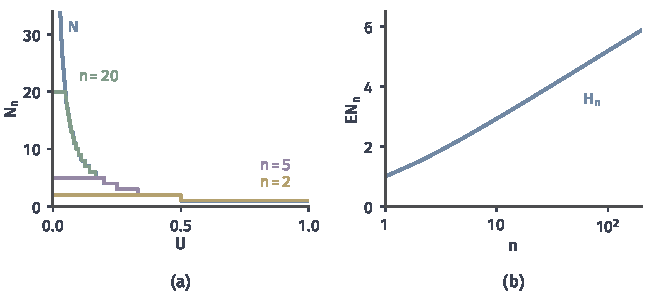
\includegraphics[width=112mm]{figures/07-probability/03-probability-limits/matplotlib/rvconv-monotone-count/figure.pdf}
 \caption{递增的计数变量$N_n=\sum_{k\leq n}\mathbf{1}_{\{U<1/k\}}$。(a)$N_n$作为$U$的函数，$n=2,5,20$（黄、紫、绿），蓝色台阶是极限$N=\lceil1/U\rceil-1$；各条台阶在$N\leq n$处与极限重合，只在$U$接近$0$处被截平。(b)$\mathbb{E}[N_n]=H_n=\sum_{k\leq n}1/k$，横轴为对数刻度。}
 \label{fig:rvconv-monotone-count}
\end{BookInlineFigure}

图~\ref{fig:rvconv-monotone-count}(a)中，$N_n$是极限$N$在高度$n$处的截平，截平的部分只在$U<1/n$这一小段上。随着$n$增大，截平的位置抬高，$N_n$下方的面积$H_n$一点一点地逼近$N$下方的面积。$N$在$U\to0$时像$1/U$那样增长，面积发散，(b)中$H_n\approx\ln n+0.577$随之无界增长。单调收敛定理正确地给出$\mathbb{E}[N]=+\infty$，它不需要极限可积。

\paragraph{单调性为何保留全部质量}
递增列不会丢掉期望的原因可以这样理解：每个$X_n$都在极限$X$的下方，且越来越贴近它。$X$的期望由它在各处的取值累积而成，任何一块有贡献的区域，迟早都会被$X_n$从下方填满，不存在“先出现、后消失”的贡献。

仅有非负性不够。$Y_n$非负且几乎必然趋于$0$，但不单调：$Y_n$在$\{U<1/n\}$上取$n$，在$Y_{n+1}$时这一块的大部分归零，又在更窄的$\{U<1/(n+1)\}$上取更大的值。图~\ref{fig:rvconv-spike-mass}在取值的数轴上画出它的分布：$Y_n$把质量$1/n$放在远处的$n$上，这一小块质量对均值的贡献恒为$n\cdot1/n=1$。随着$n$增大，这块质量越来越小、越来越远，极限中它消失了，它对均值的贡献却始终在。

\begin{BookInlineFigure}
 \centering
 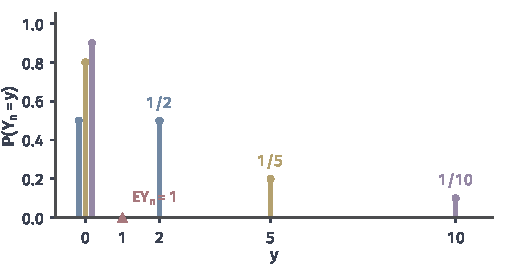
\includegraphics[width=86mm]{figures/07-probability/03-probability-limits/matplotlib/rvconv-spike-mass/figure.pdf}
 \caption{$Y_n=n\,\mathbf{1}_{\{U<1/n\}}$的分布，$n=2,5,10$（蓝、黄、紫）：质量$1-1/n$在$0$，质量$1/n$在$n$（$0$处的柱略微错开）。红三角是均值$\mathbb{E}[Y_n]=1$，对每个$n$都相同。}
 \label{fig:rvconv-spike-mass}
\end{BookInlineFigure}

\paragraph{递减的情形}
对递减列，单调性还需要配合可积性。若$X_n\geq0$递减到$X$且$\mathbb{E}[X_1]<\infty$，则$X_1-X_n$非负递增到$X_1-X$，对它用定理~\ref{thm:rvconv-monotone}，再从两边减去有限的$\mathbb{E}[X_1]$，得到$\mathbb{E}[X_n]\downarrow\mathbb{E}[X]$。

$\mathbb{E}[X_1]<\infty$不能省。取$X_n=U^{-1}\mathbf{1}_{\{U<1/n\}}$，它在$U>0$时递减到$0$，但对每个$n$，
\[
 \mathbb{E}[X_n]=\int_0^{1/n}\frac{\mathrm{d}u}{u}=+\infty .
\]
极限的期望是$0$，各项的期望都是$+\infty$。无穷减无穷没有意义，单调收敛定理只能用于递增的方向。

\subsection{Fatou引理}
\label{sec:rvconv-fatou}

不单调的非负列中，期望可以在极限里丢失，$Y_n$就是例子。但丢失只有一个方向：非负变量的质量可以逃到远处而消失，不能凭空产生。Fatou引理把这个单向的控制写成不等式。

\begin{theorem}[Fatou引理]
\label{thm:rvconv-fatou}
设随机变量$X_n\geq0$几乎必然成立，则
\begin{equation}
 \mathbb{E}\Bigl[\liminf_{n\to\infty}X_n\Bigr]\leq\liminf_{n\to\infty}\mathbb{E}[X_n] .
 \label{eq:rvconv-fatou}
\end{equation}
\end{theorem}

\begin{proof}
令$G_n=\inf_{k\geq n}X_k$。它非负，随$n$递增，极限是$\liminf_nX_n$。由定理~\ref{thm:rvconv-monotone}，
\[
 \mathbb{E}[G_n]\to\mathbb{E}\Bigl[\liminf_{n\to\infty}X_n\Bigr] .
\]

另一方面，对每个$k\geq n$都有$G_n\leq X_k$，所以$\mathbb{E}[G_n]\leq\mathbb{E}[X_k]$，对$k\geq n$取下确界，得到
\[
 \mathbb{E}[G_n]\leq\inf_{k\geq n}\mathbb{E}[X_k] .
\]
令$n\to\infty$，左边趋于式~\eqref{eq:rvconv-fatou}的左边，右边趋于它的右边。
\end{proof}

证明把一般的列换成它的尾部下确界，后者是递增的，于是可以用单调收敛。下确界只会比每一项都小，这就是不等式只有一个方向的来源。

\paragraph{严格不等号}
对$Y_n$，每条$U>0$的记录上$Y_n\to0$，所以式~\eqref{eq:rvconv-fatou}的两边是
\[
 \mathbb{E}\Bigl[\liminf_{n\to\infty}Y_n\Bigr]=0,\qquad \liminf_{n\to\infty}\mathbb{E}[Y_n]=1 .
\]
不等号严格成立，差额$1$正是逃到远处的那一块质量的贡献。概率越来越小、幅值越来越大的变量，总可以这样让极限的期望小于期望的极限。

\paragraph{非负性的作用}
把$Y_n$换成$-Y_n$，变量非正，几乎必然趋于$0$，而$\mathbb{E}[-Y_n]=-1$。这时
\[
 \mathbb{E}\Bigl[\liminf_{n\to\infty}(-Y_n)\Bigr]=0>-1=\liminf_{n\to\infty}\mathbb{E}[-Y_n] ,
\]
不等式反向。负的大值逃到远处时，带走的是负的贡献，极限的期望反而变大。所以Fatou引理需要下方的控制：非负，或者更一般地$X_n\geq-G$且$\mathbb{E}[G]<\infty$（对$X_n+G$用引理）。

\paragraph{极限的可积性}
Fatou引理最常用的形式是给极限的期望一个上界。若$X_n\xrightarrow{\mathrm{a.s.}}X$且$\sup_n\mathbb{E}[\lvert X_n\rvert]\leq C$，对$\lvert X_n\rvert$用式~\eqref{eq:rvconv-fatou}，得到
\begin{equation}
 \mathbb{E}[\lvert X\rvert]\leq\liminf_{n\to\infty}\mathbb{E}[\lvert X_n\rvert]\leq C .
 \label{eq:rvconv-fatou-bound}
\end{equation}
各项的平均绝对值一致有界时，极限必然可积。它只给出不等式，并不说明$\mathbb{E}[X_n]$收敛到$\mathbb{E}[X]$：$Y_n$满足$C=1$，极限的期望$0$严格小于$1$。

\subsection{支配收敛}
\label{sec:rvconv-dominated}

要得到等式，需要阻止质量逃逸。最直接的办法是给整列找一个共同的上界，并要求这个上界本身可积：所有变量都被关在同一个“有限面积”的笼子里。

\begin{theorem}[支配收敛定理]
\label{thm:rvconv-dominated}
设$X_n\xrightarrow{\mathrm{a.s.}}X$，并存在随机变量$G$，使$\mathbb{E}[G]<\infty$且对每个$n$都有$\lvert X_n\rvert\leq G$几乎必然成立。则$X$可积，且
\begin{equation}
 \lim_{n\to\infty}\mathbb{E}\bigl[\lvert X_n-X\rvert\bigr]=0,\qquad \lim_{n\to\infty}\mathbb{E}[X_n]=\mathbb{E}[X] .
 \label{eq:rvconv-dominated}
\end{equation}
\end{theorem}

\begin{proof}
取极限得$\lvert X\rvert\leq G$几乎必然，所以$X$可积，并且$\lvert X_n-X\rvert\leq2G$。于是$2G-\lvert X_n-X\rvert$非负，几乎必然趋于$2G$。由Fatou引理，
\[
 \mathbb{E}[2G]\leq\liminf_{n\to\infty}\mathbb{E}\bigl[2G-\lvert X_n-X\rvert\bigr]=\mathbb{E}[2G]-\limsup_{n\to\infty}\mathbb{E}\bigl[\lvert X_n-X\rvert\bigr] .
\]

$\mathbb{E}[2G]$有限，可以从两边消去，得到$\limsup_n\mathbb{E}[\lvert X_n-X\rvert]\leq0$，即平均绝对误差趋于零。最后，
\[
 \bigl\lvert\mathbb{E}[X_n]-\mathbb{E}[X]\bigr\rvert\leq\mathbb{E}\bigl[\lvert X_n-X\rvert\bigr]\to0 .
\]
\end{proof}

证明的关键是把误差$\lvert X_n-X\rvert$翻成$2G$减去它，后者非负，Fatou引理就从“只能变小”的单向控制变成了对误差的控制。可积性$\mathbb{E}[G]<\infty$用在消去$\mathbb{E}[2G]$这一步。

\paragraph{有界收敛}
概率空间的总质量为一，常数是可积的。所以若$\lvert X_n\rvert\leq c$对某个常数$c$成立，支配条件自动满足，这称为\term{有界收敛定理}（bounded convergence theorem）。累计最大值满足$0\leq M_n\leq1$，于是
\[
 \mathbb{E}[M_n]=\frac{n}{n+1}\to1=\mathbb{E}[1] .
\]
在一般测度空间上，常数在总测度无限时不可积，有界收敛不能这样直接得到。

\paragraph{依概率收敛下的支配收敛}
定理中的几乎必然收敛可以减弱为依概率收敛。设$X_n\xrightarrow{\mathbb{P}}X$，$\lvert X_n\rvert\leq G$，$\mathbb{E}[G]<\infty$，记$a_n=\mathbb{E}[\lvert X_n-X\rvert]$。由定理~\ref{thm:rvconv-subsequence}，有子列几乎必然收敛到$X$，取极限得$\lvert X\rvert\leq G$，$X$可积。

再看数列$(a_n)$的任意子列。由定理~\ref{thm:rvconv-subsequence-criterion}，它有进一步的子列使$X_n$几乎必然收敛到$X$，对这个子列用定理~\ref{thm:rvconv-dominated}，相应的$a_n$趋于零。一个实数列的每个子列都有趋于零的进一步子列，整个数列就趋于零，所以$a_n\to0$。

\paragraph{共同上界与包络}
$Y_n$为什么不满足定理？任何共同上界$G$都不小于包络$\sup_nY_n$。对$U(\omega)>0$，$Y_n(\omega)=n$当且仅当$n<1/U(\omega)$，所以包络就是第~\ref{sec:rvconv-monotone}小节的计数变量：
\[
 \sup_nY_n=\Bigl\lceil\frac1U\Bigr\rceil-1=N,\qquad \mathbb{E}[N]=+\infty .
\]
包络不可积，任何共同上界也不可积，支配收敛定理不适用，结论也确实不成立。

$Z_n=\sqrt n\,\mathbf{1}_{\{U<1/n\}}$的包络是$\sqrt N$。$N=n$当且仅当$1/(n+1)\leq U<1/n$，概率为$1/(n(n+1))$，所以
\[
 \mathbb{E}\bigl[\sqrt N\bigr]=\sum_{n=1}^{\infty}\frac{\sqrt n}{n(n+1)}=\sum_{n=1}^{\infty}\frac{1}{\sqrt n\,(n+1)}\approx1.860 .
\]
包络可积，支配收敛定理给出$\mathbb{E}[Z_n]\to0$，与直接计算的$n^{-1/2}$一致。

\begin{BookInlineFigure}
 \centering
 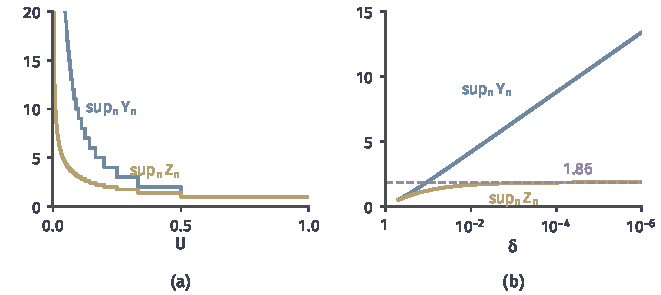
\includegraphics[width=112mm]{figures/07-probability/03-probability-limits/matplotlib/rvconv-envelope/figure.pdf}
 \caption{两族稀有大值的包络。(a)$\sup_nY_n=\lceil1/U\rceil-1$（蓝）与$\sup_nZ_n=\sqrt{\lceil1/U\rceil-1}$（黄）作为$U$的函数。(b)从$\delta$到$1$的积分随$\delta\to0$的变化，横轴为对数刻度且向右递减：蓝线按$\ln(1/\delta)$无界增长，黄线趋于$\mathbb{E}[\sqrt N]\approx1.86$（紫色虚线）。}
 \label{fig:rvconv-envelope}
\end{BookInlineFigure}

图~\ref{fig:rvconv-envelope}比较两个包络。两者在$U\to0$时都趋于无穷，差别在于增长的快慢：$\sup_nY_n$像$1/U$，下方面积发散；$\sup_nZ_n$像$U^{-1/2}$，下方面积有限。共同上界控制的不是单个变量，而是整族变量在稀有区域上能取到的最大值。

\paragraph{共同上界控制了什么}
共同可积上界的作用可以写成一个统一的尾部估计。若$\lvert X_n\rvert\leq G$，则$\{\lvert X_n\rvert>M\}\subseteq\{G>M\}$，在这个事件上$\lvert X_n\rvert\leq G$，所以
\begin{equation}
 \sup_n\mathbb{E}\bigl[\lvert X_n\rvert\,\mathbf{1}_{\{\lvert X_n\rvert>M\}}\bigr]\leq\mathbb{E}\bigl[G\,\mathbf{1}_{\{G>M\}}\bigr] .
 \label{eq:rvconv-envelope-tail}
\end{equation}
右边是单个可积变量的尾部贡献，$M\to\infty$时由支配收敛趋于零。共同上界真正做到的，是让整族变量在大取值处的贡献一起变小。下一小节把这一点单独拿出来作为条件。

\subsection{一致可积性}
\label{sec:rvconv-uniform-integrability}

$Y_n$的问题是平均被越来越稀有的大值维持着。要排除这种情形，应当要求大取值区域上的贡献对整族变量一致地小，而不必要求有一个共同的上界。

\begin{definition}[一致可积]
\label{def:rvconv-ui}
设$\{X_i:i\in I\}$是一族可积随机变量。若
\begin{equation}
 \lim_{M\to\infty}\ \sup_{i\in I}\ \mathbb{E}\bigl[\lvert X_i\rvert\,\mathbf{1}_{\{\lvert X_i\rvert>M\}}\bigr]=0 ,
 \label{eq:rvconv-ui}
\end{equation}
称这族变量\term{一致可积}（uniformly integrable）。
\end{definition}

单个可积变量$X$总满足这个条件：$\lvert X\rvert\mathbf{1}_{\{\lvert X\rvert>M\}}$被$\lvert X\rvert$控制，且在$\lvert X\rvert<\infty$处随$M\to\infty$趋于零，由支配收敛定理，它的期望趋于零。有限个可积变量也一致可积，对每个变量分别取$M$再取最大的那个即可。一致可积性的内容在于无穷多个变量同时满足，即同一个$M$对整族有效。

\paragraph{贯穿例子}
$Y_n$不一致可积。对任意$M$，当$n>M$时$\{Y_n>M\}=\{U<1/n\}$，所以
\[
 \mathbb{E}\bigl[Y_n\mathbf{1}_{\{Y_n>M\}}\bigr]=n\cdot\frac1n=1,\qquad
 \sup_n\mathbb{E}\bigl[Y_n\mathbf{1}_{\{Y_n>M\}}\bigr]=1 .
\]
无论阈值抬多高，总有某个$Y_n$把全部平均放在阈值之上。

$Z_n$一致可积。只有$\sqrt n>M$时$\{Z_n>M\}$才非空，此时它的贡献是$\sqrt n\cdot1/n=1/\sqrt n<1/M$，所以
\[
 \sup_n\mathbb{E}\bigl[Z_n\mathbf{1}_{\{Z_n>M\}}\bigr]\leq\frac1M\to0 .
\]
累计最大值在$[0,1]$中取值，$M\geq1$时贡献为零。图~\ref{fig:rvconv-ui-tails}画出三族的上确界随$M$的变化。

\begin{BookInlineFigure}
 \centering
 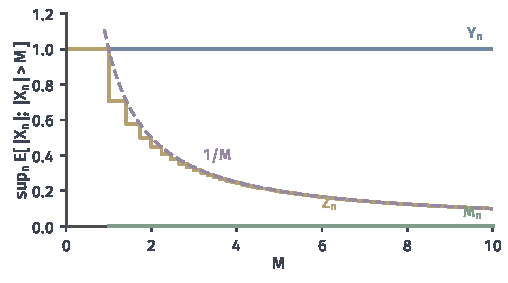
\includegraphics[width=86mm]{figures/07-probability/03-probability-limits/matplotlib/rvconv-ui-tails/figure.pdf}
 \caption{大取值区域上的一致贡献$\sup_n\mathbb{E}[\lvert X_n\rvert;\lvert X_n\rvert>M]$随阈值$M$的变化。蓝线：$Y_n$，恒为$1$，不一致可积。黄色台阶：$Z_n$，等于$1/\sqrt{\lfloor M^{2}\rfloor+1}$。紫色虚线：二阶矩给出的上界$\sup_n\mathbb{E}[Z_n^{2}]/M=1/M$。绿线：$M_n$，$M\geq1$时为零。}
 \label{fig:rvconv-ui-tails}
\end{BookInlineFigure}

\paragraph{判据}
直接验证式~\eqref{eq:rvconv-ui}往往不方便。下面三条比较常用的条件说明：共同可积上界和高于一阶的一致矩界都足够，而一阶矩一致有界本身不够。

\begin{theorem}[一致可积的充分条件]
\label{thm:rvconv-ui-criteria}
设$\{X_i:i\in I\}$是一族随机变量。
\begin{enumerate}
 \item 若存在$G$，$\mathbb{E}[G]<\infty$，使$\lvert X_i\rvert\leq G$对每个$i$几乎必然成立，则这族变量一致可积。
 \item 若存在$p>1$与$K<\infty$，使$\mathbb{E}[\lvert X_i\rvert^{p}]\leq K$对每个$i$成立，则这族变量一致可积，且
 \begin{equation}
  \sup_{i\in I}\mathbb{E}\bigl[\lvert X_i\rvert\,\mathbf{1}_{\{\lvert X_i\rvert>M\}}\bigr]\leq\frac{K}{M^{p-1}} .
  \label{eq:rvconv-ui-moment}
 \end{equation}
 \item 仅有$\sup_i\mathbb{E}[\lvert X_i\rvert]<\infty$不能推出一致可积。
\end{enumerate}
\end{theorem}

\begin{proof}
第1条即式~\eqref{eq:rvconv-envelope-tail}。

第2条。在$\{\lvert X_i\rvert>M\}$上，$\lvert X_i\rvert^{1-p}<M^{1-p}$，所以
\[
 \lvert X_i\rvert=\lvert X_i\rvert^{p}\cdot\lvert X_i\rvert^{1-p}\leq\frac{\lvert X_i\rvert^{p}}{M^{p-1}} .
\]
乘以$\mathbf{1}_{\{\lvert X_i\rvert>M\}}$再取期望，右边的期望不超过$\mathbb{E}[\lvert X_i\rvert^{p}]\leq K$，即得式~\eqref{eq:rvconv-ui-moment}。$p>1$保证右边随$M\to\infty$趋于零。

第3条。$Y_n$满足$\mathbb{E}[Y_n]=1$，但上面已算出它不一致可积。
\end{proof}

第2条中$p>1$是关键。$p$阶矩有界意味着大取值必须付出更高的代价：取值为$y$的部分在$p$阶矩中按$y^{p}$计入，在平均中只按$y$计入，所以平均的尾部被$p$阶矩以$M^{1-p}$的速度压住。$p=1$时这个比例是$1$，没有压缩，$Y_n$就钻了这个空子。$Z_n$满足$\mathbb{E}[Z_n^{2}]=1$，第2条给出上界$1/M$，正是图~\ref{fig:rvconv-ui-tails}中的紫色虚线。

同样的论证适用于任何增长快于线性的函数。若$\varphi\geq0$满足$\varphi(t)/t\to\infty$（$t\to\infty$），且$\sup_i\mathbb{E}[\varphi(\lvert X_i\rvert)]\leq K$，则在$\{\lvert X_i\rvert>M\}$上
\[
 \lvert X_i\rvert=\varphi(\lvert X_i\rvert)\cdot\frac{\lvert X_i\rvert}{\varphi(\lvert X_i\rvert)}\leq\varphi(\lvert X_i\rvert)\,\sup_{t>M}\frac{t}{\varphi(t)} ,
\]
于是尾部贡献不超过$K\sup_{t>M}t/\varphi(t)$，它随$M\to\infty$趋于零。例如$\varphi(t)=t\ln(1+t)$，它只比一阶矩多一个对数因子。反过来，每个一致可积族都存在这样的$\varphi$，这一方向的证明需要构造$\varphi$，篇幅较长，读者可查阅~\scite{math-kallenberg2021probability}。

\paragraph{小事件上的一致控制}
一致可积还有一个等价的说法：平均有界，并且在概率很小的事件上，整族变量的贡献一致地小。它把“大取值”换成了“小事件”，在证明中更方便。

\begin{lemma}[一致可积的等价刻画]
\label{lem:rvconv-ui-small-sets}
一族随机变量$\{X_i:i\in I\}$一致可积，当且仅当以下两条同时成立：
\begin{enumerate}
 \item $\sup_{i\in I}\mathbb{E}[\lvert X_i\rvert]<\infty$；
 \item 对每个$\eta>0$，存在$\delta>0$，使对每个满足$\mathbb{P}(A)<\delta$的事件$A$，
 \begin{equation}
  \sup_{i\in I}\mathbb{E}\bigl[\lvert X_i\rvert\,\mathbf{1}_{A}\bigr]<\eta .
  \label{eq:rvconv-ui-small-sets}
 \end{equation}
\end{enumerate}
\end{lemma}

\begin{proof}
必要性。把事件$A$按$\lvert X_i\rvert$是否超过$M$分成两块，第二块上$\lvert X_i\rvert\leq M$，所以
\[
 \mathbb{E}\bigl[\lvert X_i\rvert\,\mathbf{1}_{A}\bigr]\leq\mathbb{E}\bigl[\lvert X_i\rvert\,\mathbf{1}_{\{\lvert X_i\rvert>M\}}\bigr]+M\,\mathbb{P}(A) .
\]
给定$\eta>0$，先取$M$使第一项对所有$i$都小于$\eta/2$，再取$\delta=\eta/(2M)$，则$\mathbb{P}(A)<\delta$时左边小于$\eta$。取$A=\Omega$，第一项小于$\eta/2$，第二项是$M$，得到第1条。

充分性。记$C=\sup_i\mathbb{E}[\lvert X_i\rvert]$。由Markov不等式，
\[
 \mathbb{P}\bigl(\lvert X_i\rvert>M\bigr)\leq\frac{C}{M}\qquad\text{对每个 }i .
\]
给定$\eta$，取第2条中的$\delta$，再取$M>C/\delta$，则每个事件$\{\lvert X_i\rvert>M\}$的概率都小于$\delta$，由式~\eqref{eq:rvconv-ui-small-sets}，其上的贡献小于$\eta$，且对所有$i$同时成立。
\end{proof}

充分性中第1条不可缺：它保证事件$\{\lvert X_i\rvert>M\}$对整族一致地小，第2条才能用上。这个刻画说明，一致可积排除的正是“把平均藏在越来越小的事件里”。$Y_n$在概率$1/n$的事件上放下整份平均$1$，第2条对它不成立。

\subsection{\texorpdfstring{$L^{1}$}{L1}收敛的判据}
\label{sec:rvconv-l1-criterion}

现在可以回答本节开头的问题。依概率收敛缺的是尾部控制，一致可积恰好补上它，而且补得不多不少：在依概率收敛的前提下，$L^{1}$收敛与一致可积等价。

\begin{theorem}[Vitali收敛定理]
\label{thm:rvconv-vitali}
设$X_n\xrightarrow{\mathbb{P}}X$，且$\{X_n\}$一致可积。则$X$可积，且
\begin{equation}
 \lim_{n\to\infty}\mathbb{E}\bigl[\lvert X_n-X\rvert\bigr]=0,\qquad \lim_{n\to\infty}\mathbb{E}[X_n]=\mathbb{E}[X] .
 \label{eq:rvconv-vitali}
\end{equation}
\end{theorem}

这一结论称为\term{Vitali收敛定理}（Vitali convergence theorem）。卷四对有限测度空间的依测度收敛给出了一个按小区域估计的证明。这里换一种在概率论中更常用的写法：把每个变量截断成有界变量，有界部分用有界收敛，截掉的尾部用一致可积。对$M>0$，令
\[
 \varphi_M(x)=\max\{-M,\min\{x,M\}\} ,
\]
即把$x$限制在$[-M,M]$内。它满足两条性质：截断不会拉大两点的距离，截断误差只出现在阈值之外，
\[
 \lvert\varphi_M(x)-\varphi_M(y)\rvert\leq\lvert x-y\rvert,\qquad
 \lvert x-\varphi_M(x)\rvert\leq\lvert x\rvert\,\mathbf{1}_{\{\lvert x\rvert>M\}} .
\]
后一式左边等于$\max\{\lvert x\rvert-M,0\}$。

\begin{BookInlineFigure}
 \centering
 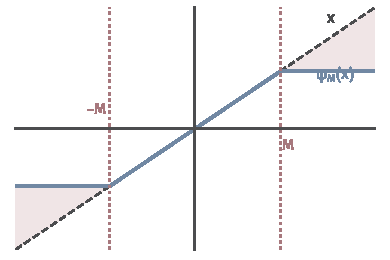
\includegraphics[width=66mm]{figures/07-probability/03-probability-limits/matplotlib/rvconv-truncation/figure.pdf}
 \caption{截断函数$\varphi_M$（蓝线，$M=2$）与恒等函数（灰色虚线）。两者只在$\lvert x\rvert>M$处不同，浅红区域的竖直高度就是截断误差$\lvert x-\varphi_M(x)\rvert=(\lvert x\rvert-M)^{+}$。}
 \label{fig:rvconv-truncation}
\end{BookInlineFigure}

图~\ref{fig:rvconv-truncation}画出截断误差的位置：它只出现在阈值之外，而一致可积说的正是阈值之外的贡献一致地小。

\begin{proof}
先证$X$可积。由引理~\ref{lem:rvconv-ui-small-sets}，$C=\sup_n\mathbb{E}[\lvert X_n\rvert]<\infty$。由定理~\ref{thm:rvconv-subsequence}，有子列$X_{n_k}\xrightarrow{\mathrm{a.s.}}X$，再由式~\eqref{eq:rvconv-fatou-bound}，$\mathbb{E}[\lvert X\rvert]\leq C$。

再估计误差。固定$M>0$，在$X_n$与$X$之间插入截断，由三角不等式，
\[
 \lvert X_n-X\rvert\leq\lvert X_n-\varphi_M(X_n)\rvert+\lvert\varphi_M(X_n)-\varphi_M(X)\rvert+\lvert\varphi_M(X)-X\rvert .
\]
取期望，逐项处理。

第一项是截掉的尾部，由截断误差的估计，
\[
 \mathbb{E}\bigl[\lvert X_n-\varphi_M(X_n)\rvert\bigr]\leq\tau(M),\qquad \tau(M)=\sup_k\mathbb{E}\bigl[\lvert X_k\rvert\,\mathbf{1}_{\{\lvert X_k\rvert>M\}}\bigr] .
\]
第三项同理不超过$\mathbb{E}[\lvert X\rvert\mathbf{1}_{\{\lvert X\rvert>M\}}]$。

第二项是有界部分。由$\varphi_M$的第一条性质，截断后的误差不超过原误差，所以$\varphi_M(X_n)\xrightarrow{\mathbb{P}}\varphi_M(X)$；同时它不超过$2M$。由依概率收敛下的有界收敛（第~\ref{sec:rvconv-dominated}小节），第二项的期望趋于零。于是
\[
 \limsup_{n\to\infty}\mathbb{E}\bigl[\lvert X_n-X\rvert\bigr]\leq\tau(M)+\mathbb{E}\bigl[\lvert X\rvert\,\mathbf{1}_{\{\lvert X\rvert>M\}}\bigr] .
\]

左边与$M$无关。令$M\to\infty$，第一项由一致可积趋于零，第二项因$X$可积而趋于零，所以平均绝对误差趋于零。期望的收敛与支配收敛定理的证明末尾相同。
\end{proof}

三个部分各有分工：依概率收敛只管有界的中间部分，一致可积管住所有$X_n$的尾部，$X$的可积性管住极限的尾部。缺了一致可积，第一项不能对所有$n$同时变小，$Y_n$就是这种情形：$\tau(M)=1$，误差停在$1$。

用贯穿例子核对。$Z_n\xrightarrow{\mathbb{P}}0$且一致可积，定理给出$\mathbb{E}[Z_n]\to0$，与直接计算的$n^{-1/2}$一致。移动区块与$\xi_n$都只取$0$和$1$，由第1条判据（$G=1$）一致可积，它们依概率收敛到$0$，所以也$L^{1}$收敛到$0$，与第~\ref{sec:rvconv-lp}小节的计算一致。

\paragraph{反方向}
$L^{1}$收敛的列一定一致可积，所以一致可积不只是充分条件。

\begin{theorem}[$L^{1}$收敛蕴含一致可积]
\label{thm:rvconv-l1-ui}
若$X_n\xrightarrow{L^{1}}X$，则$\{X_n\}$一致可积，且$X_n\xrightarrow{\mathbb{P}}X$。
\end{theorem}

\begin{proof}
依概率收敛是定理~\ref{thm:rvconv-implications}的第2条。一致可积用引理~\ref{lem:rvconv-ui-small-sets}验证。

平均有界。由三角不等式，
\[
 \mathbb{E}[\lvert X_n\rvert]\leq\mathbb{E}[\lvert X\rvert]+\mathbb{E}[\lvert X_n-X\rvert] ,
\]
右边第二项趋于零，所以左边有界。

小事件上的控制：对任意事件$A$，
\[
 \mathbb{E}\bigl[\lvert X_n\rvert\,\mathbf{1}_{A}\bigr]\leq\mathbb{E}\bigl[\lvert X\rvert\,\mathbf{1}_{A}\bigr]+\mathbb{E}\bigl[\lvert X_n-X\rvert\bigr] .
\]
给定$\eta>0$，取$N$使$n\geq N$时$\mathbb{E}[\lvert X_n-X\rvert]<\eta/2$。有限族$\{X,X_1,\dots,X_{N-1}\}$一致可积，由引理~\ref{lem:rvconv-ui-small-sets}，存在$\delta$，使$\mathbb{P}(A)<\delta$时其中每个变量在$A$上的贡献都小于$\eta/2$。

于是$\mathbb{P}(A)<\delta$时，$n<N$的项在$A$上的贡献小于$\eta/2$，$n\geq N$的项由上式小于$\eta/2+\eta/2=\eta$。
\end{proof}

两个定理合起来：在$X_n\xrightarrow{\mathbb{P}}X$的前提下，
\begin{equation}
 X_n\xrightarrow{L^{1}}X\quad\Longleftrightarrow\quad\{X_n\}\text{ 一致可积} .
 \label{eq:rvconv-l1-iff}
\end{equation}
依概率收敛与一致可积分别补上了第~\ref{sec:rvconv-comparison}节所说的两种缺陷中的一种：前者保证超差的机会消失，后者保证超差的大小不能维持平均。

\paragraph{\texorpdfstring{$L^{p}$}{Lp}收敛}
同样的判据适用于$p$阶矩。设$X_n\xrightarrow{\mathbb{P}}X$，$\{\lvert X_n\rvert^{p}\}$一致可积。由Fatou引理$X$的$p$阶矩有限，再由
\[
 \lvert X_n-X\rvert^{p}\leq2^{p-1}\bigl(\lvert X_n\rvert^{p}+\lvert X\rvert^{p}\bigr)
\]
和引理~\ref{lem:rvconv-ui-small-sets}，$\{\lvert X_n-X\rvert^{p}\}$也一致可积。它依概率收敛到$0$，由定理~\ref{thm:rvconv-vitali}，$\mathbb{E}[\lvert X_n-X\rvert^{p}]\to0$，即$X_n\xrightarrow{L^{p}}X$。

用$Z_n$核对$p=2$。$\{Z_n^{2}\}=\{n\,\mathbf{1}_{\{U<1/n\}}\}=\{Y_n\}$不一致可积，所以判据不能给出$L^{2}$收敛，而由式~\eqref{eq:rvconv-spike-moments}，$\mathbb{E}[Z_n^{2}]=1$，$Z_n$确实不$L^{2}$收敛。同一列变量$\{Z_n\}$一致可积而$\{Z_n^{2}\}$不一致可积，这正是第~\ref{sec:rvconv-comparison}节中$L^{1}$收敛与$L^{2}$收敛的分界。

\paragraph{期望收敛与平均误差}
最后要区分两件事：$\mathbb{E}[\lvert X_n-X\rvert]\to0$与$\mathbb{E}[X_n]\to\mathbb{E}[X]$。前者推出后者，后者推不出前者，因为期望是有符号的，正负误差可以互相抵消。取
\[
 W_n=n\,\mathbf{1}_{\{U<1/(2n)\}}-n\,\mathbf{1}_{\{1/(2n)\leq U<1/n\}} .
\]
它在$U>0$时最终为零，$W_n\xrightarrow{\mathrm{a.s.}}0$。正负两块各贡献$\pm1/2$，所以
\[
 \mathbb{E}[W_n]=\frac12-\frac12=0,\qquad \mathbb{E}\bigl[\lvert W_n\rvert\bigr]=\frac12+\frac12=1 .
\]

\begin{BookInlineFigure}
 \centering
 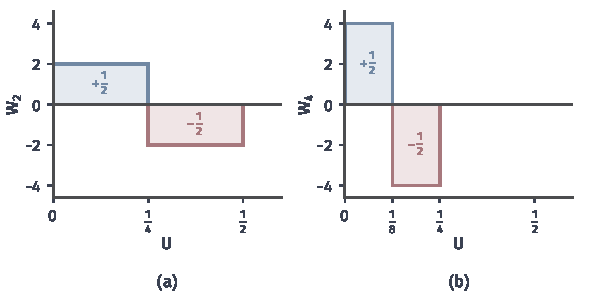
\includegraphics[width=100mm]{figures/07-probability/03-probability-limits/matplotlib/rvconv-signed-cancel/figure.pdf}
 \caption{正负抵消的变量$W_n$作为$U$的函数。浅蓝块是正的部分，面积$1/2$；浅红块是负的部分，面积$1/2$。(a)$n=2$。(b)$n=4$。期望恒为$0$，平均绝对误差恒为$1$。}
 \label{fig:rvconv-signed-cancel}
\end{BookInlineFigure}

图~\ref{fig:rvconv-signed-cancel}中正负两块面积相等，期望恰好是零，与极限$0$的期望相同；但两块的绝对面积加起来是$1$，平均绝对误差没有消失。$\{W_n\}$不一致可积，与$Y_n$同理。期望收敛只是一个数的收敛，平均绝对误差的消失才是误差本身在平均意义下的消失。

对非负变量，抵消不会发生，两者等价。

\begin{lemma}[Scheffé引理]
\label{lem:rvconv-scheffe}
设$X_n\geq0$，$X_n\xrightarrow{\mathbb{P}}X$，$\mathbb{E}[X]<\infty$，且$\mathbb{E}[X_n]\to\mathbb{E}[X]$。则$\mathbb{E}[\lvert X_n-X\rvert]\to0$。
\end{lemma}

\begin{proof}
依概率收敛的子列几乎必然收敛，所以$X\geq0$几乎必然。把绝对值拆成正部与负部，$\lvert a\rvert=a+2\max\{-a,0\}$，取$a=X_n-X$，得到
\[
 \mathbb{E}\bigl[\lvert X_n-X\rvert\bigr]=\bigl(\mathbb{E}[X_n]-\mathbb{E}[X]\bigr)+2\,\mathbb{E}\bigl[(X-X_n)^{+}\bigr] .
\]
第一项按假设趋于零。第二项中$0\leq(X-X_n)^{+}\leq X$，这里用到$X_n\geq0$；$(X-X_n)^{+}$依概率收敛到$0$，又被可积的$X$控制，由依概率收敛下的支配收敛，它的期望趋于零。
\end{proof}

这个结论称为\term{Scheffé引理}（Scheffé's lemma）。非负性让负部被极限$X$从上方压住，正部的大小又由期望之差决定，抵消无处藏身。$Y_n$也是非负的，但$\mathbb{E}[Y_n]=1$不趋于$\mathbb{E}[0]=0$，引理的条件不满足，这与它不$L^{1}$收敛一致。


\section{本章小结}
\label{sec:rvconv-summary}

本章在同一个概率空间上研究随机误差$X_n-X$怎样趋于零。三种收敛方式对应三种要求：几乎必然收敛看每条记录上的数列，允许一个零概率的例外集；依概率收敛看每一项超差事件的概率；$L^{p}$收敛看误差$p$次幂的平均。表~\ref{tab:rvconv-summary}列出它们各自控制和放过的东西。

\begin{BookInlineTable}
 \centering
 \begin{tabular}{@{}lll@{}}
  \toprule
  收敛方式 & 要求 & 不控制 \\
  \midrule
  几乎必然 & 几乎每条记录最终不再超差 & 超差的幅度 \\
  依概率 & 每项超差的概率趋于零 & 反复超差、超差的幅度 \\
  $L^{p}$ & 误差$p$次幂的期望趋于零 & 同一记录的反复超差 \\
  \bottomrule
 \end{tabular}
 \caption{三种收敛方式的要求与盲点。}
 \label{tab:rvconv-summary}
\end{BookInlineTable}

几乎必然收敛与$L^{p}$收敛都推出依概率收敛，较高阶的$L^{p}$收敛推出较低阶的。反方向的失败有两种来源。稀有大值$Y_n$、$Z_n$缺的是尾部控制：超差越来越少，但每次越来越大。移动区块$B_n$与独立示性变量$\xi_n$缺的是整列的逐样本控制：超差事件越来越小，却在每条记录上反复出现。图~\ref{fig:rvconv-implications}汇总了这些关系，以及补上缺陷后可以反向推出的结论。

\begin{BookInlineFigure}
 \centering
 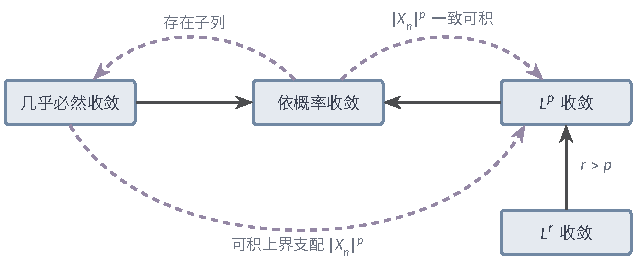
\includegraphics[width=108mm]{figures/07-probability/03-probability-limits/tikz/rvconv-implications/figure.pdf}
 \caption{同一概率空间上收敛方式之间的关系，$1\leq p<r<\infty$。深灰实线箭头总是成立；紫色虚线箭头在所标条件下成立：依概率收敛的列存在几乎必然收敛的子列，依概率收敛加上$\{\lvert X_n\rvert^{p}\}$一致可积推出$L^{p}$收敛，几乎必然收敛加上$\lvert X_n\rvert^{p}$有共同可积上界推出$L^{p}$收敛。}
 \label{fig:rvconv-implications}
\end{BookInlineFigure}

几乎必然行为由事件的重复来判断。误差最终小于$\varepsilon$，就是超差事件只发生有限次；只需对可数个阈值检查。超差概率可以求和时，Borel–Cantelli引理不需要任何独立性就保证有限次发生；概率不可求和时，只有在独立条件下才能断言无穷多次发生，没有独立性则什么都推不出。依概率收敛的列总有几乎必然收敛的子列，而依概率收敛恰好等价于“每个子列都有几乎必然收敛的进一步子列”。

期望与极限的交换由尾部控制决定。单调递增的非负列不会丢失期望，极限期望可以为无穷。不单调时，Fatou引理只给出单向的不等式，丢失的部分是逃到远处的质量。共同的可积上界阻止质量逃逸，给出支配收敛；它真正控制的是整族变量在大取值处的贡献，把这一点单独拿出来就是一致可积性。共同上界和高于一阶的一致矩界都推出一致可积，一阶矩一致有界则不够。在依概率收敛的前提下，$L^{1}$收敛与一致可积等价。平均绝对误差的消失还要和有符号期望的收敛区分开，对非负变量两者才等价。

下一章研究独立随机变量的部分和与样本平均，检验它们怎样满足本章的这些要求：有限方差给出均方误差的估计和依概率收敛，强大数律则要用到几乎必然收敛的判别工具。本章始终要求各变量定义在同一个概率空间上，误差$X_n-X$才有意义；只比较各自的分布、不要求共同实现的收敛由第~\ref{chap:weak-convergence-of-distributions}章研究。

